%% thesis.tex 2014/04/11
\documentclass{ucbthesis}
\usepackage[backend=bibtex,citestyle=authoryear-icomp,bibstyle=authoryear]{biblatex}
\addbibresource{../../mendeley_bibtex.bib}
\addbibresource{../manual_additions.bib}
\usepackage{indentfirst}
\usepackage[usenames,dvipsnames]{color}
\usepackage[pdftex]{graphicx}
\usepackage{amsmath}
\usepackage{amssymb}
\usepackage{amsthm}
\usepackage{algorithm2e}
\usepackage{booktabs}
\usepackage{url}
\usepackage{float}
\usepackage{subcaption}
\usepackage{enumitem}
\usepackage{multirow}
\usepackage[colorlinks]{hyperref}

%% Math commands
\newtheorem{theorem}{Theorem}
\newtheorem{mydef}{Definition}
\DeclareMathOperator*{\argmin}{arg\,min}
\DeclareMathOperator*{\argmax}{arg\,max}

%% Misc commands
\newcommand\gray[1]{\textcolor{Gray}{#1}}
\newcommand\todo[1]{\textcolor{BrickRed}{todo: #1}}
\def\algorithmautorefname{Algorithm}
\def\subsectionautorefname{Section}

\begin{document}
\title{Anytime Recognition of Objects and Scenes}
\author{Sergey Karayev}
\degreesemester{Fall}
\degreeyear{2014}
\degree{Doctor of Philosophy}
\chair{Professor Trevor Darrell}
\othermembers{Professor Pieter Abbeel \\Professor Ken Goldberg}
\numberofmembers{3}
\field{Computer Science}

% \maketitle
% Comment out for final.
% \approvalpage
% \copyrightpage
%!TEX root=paper/paper.tex
\begin{abstract}

Humans are capable of perceiving a scene at a glance, and obtain deeper understanding with additional time.
Similarly, visual recognition deployments should be robust to varying computational budgets.
Such situations require Anytime recognition ability, which is rarely considered in computer vision research.

We present a method for learning dynamic policies to optimize Anytime performance in visual architectures.
Our method for \emph{timely} multi-class detection aims to give the best possible performance at any single point after a start time; it is terminated at a deadline time.
Toward this goal, we formulate a dynamic, closed-loop policy that infers the contents of the image in order to decide which detector to deploy next.
Crucially, we approach this problem from the perspective of Markov Decision Processes, and use reinforcement learning techniques in learning.
We explain our effective decisions in structuring the reward function and featurizing the MDP state.
In contrast to previous work, our method significantly diverges from the predominant greedy strategies, and is able to learn to take actions with deferred values.

Experiments are conducted on the PASCAL VOC object detection dataset.
We evaluate our method with a novel \emph{costliness} measure, computed as the area under an Average Precision vs. Time curve.
If execution is stopped when only half the detectors have been run, our method obtains $66\%$ better AP than a random ordering, and $14\%$ better performance than an intelligent baseline.
On the costliness measure, our method obtains at least $11\%$ better performance.
Our method is easily extensible, as it treats detectors and classifiers as black boxes and learns from execution traces using reinforcement learning.

On classification tasks, our model sequentially orders feature computation and performs subsequent classification.
Crucially, decisions are made at test time and depend on observed data and intermediate results.
We show the applicability of this system to standard problems in scene and object recognition.
On suitable datasets, we can incorporate a semantic back-off strategy that gives maximally specific predictions for a desired level of accuracy; this provides a new view on the time course of human visual perception.
\end{abstract}

\begin{frontmatter}
    \tableofcontents
    % \listoffigures
    % \listoftables
    % %!TEX root=paper/paper.tex
\begin{acknowledgements}
It is a significant stage of life to spend five years working on a PhD degree, and I am very grateful to have worked with wonderful people during this period. First and foremost, I would like to thank my advisor Trevor Darrell, for being a great mentor to introduce me into the wonderful field of academic research and to encourage me to explore new fields and research directions. I would also like to thank Jitendra Malik, Alyosha Efros, and Ken Goldberg for high-level and interdisciplinary guidances allowing me to see beyond my otherwise limited research field.
I had never imagined a more enjoyable graduate school life before I joined Berkeley, and it is an honor to meet and work with fellow postdocs and graduate students: Oriol Vinyals, Jon Barron, Yangqing Jia, Trevor Owens, Hyun Oh Song, Ning Zhang, Judy Hoffman, Allie Janoch, Jon Long, Jeff Donahue, Evan Shelhamer, Joshua Abbott, Joseph Austerweil, Dave Golland, Matthieu Salzmann, Brian Kulis, Mario Fritz, Mario Christoudias, Ross Girshick, Sergio Guadarrama, and many others. Grad school has been unimaginably colorful with your company.
I appreciate my internship days at the Adobe and Artsy.
Last but not least, I am deeply indebted to the love and support of my parents. This thesis is dedicated to them with my sincere gratitude.
\end{acknowledgements}

\end{frontmatter}

\pagestyle{headings}
%!TEX root=paper/paper.tex
\chapter{Introduction}\label{sec:introduction}

\section{Motivation}

\PM{Perception}
It is well-known that human perception is Anytime, meaning that a scene can be described after even a short presentation.
Perception is also progressive, meaning that the quality of description increases with more time.
The progressive time course of visual perception has been confirmed by multiple studies \parencite{Vanrullen-1996,Fei-Fei-Vision-2007}, with some studies providing evidence that enhancement occurs in an ontologically meaningful way.
For example, people tend to recognize something as an animal before recognizing it as a dog \parencite{Mace-PloS-2009}.
The underlying mechanisms of this behavior are unknown, and only a few attempts have been made to explain the temporal dynamics (for instance, a promising work by \cite{Hegde-Neuro-2008} has employed the framework of sequential decision processes).

\PM{Computer applications}
Meanwhile, automated visual recognition has achieved levels of performance that allow useful real-world implementation.
We focus on two problem formulations: \emph{image classification}, in which some property of the image -- such as scene type, visual style, or even object presence -- is predicted, and \emph{object detection}, in which the location and category (or identity) of all objects in a scene is predicted.
Solutions to the two problems are often linked, as classification can be a subroutine for detection.
Our motivation is that state-of-the-art methods for classification and detection tend to be computationally expensive, insensitive to Anytime demands, and not progressively enhanced.

\PM{Application}
As real-world deployment of recognition methods grows, managing resource cost (power or compute time) becomes increasingly important.
For tasks such as personal robotics, it is crucial to be able to deploy varying levels of processing to different stimuli, depending on computational demands on the robot.
A hypothetical system for vision-based advertising, in which paying customers engage with the system to have their products detected in images on the internet, presents another example.
The system has different values (in terms of cost per click) and accuracies for different classes of objects, and the backlog of unprocessed images fluctuates based on demand and available server time.
The recognition strategy to maximize profit in such an environment should exploit all signals available to it, and the quality of detections should be Anytime, depending on the length of the queue (for example, lowering recall when queue pressure grows).

\PM{Visual Features / Classification}
For most state-of-the-art classification methods, a range of features are extracted from an image instance and used to train a classifier.
Since the feature vectors are usually very high-dimensional, linear classification methods are used most often -- for instance, logistic regression.
Features are extracted at different costs, and contribute differently to decreasing classification error.
Although it can generally be said that ``the more features, the better,'' high accuracy can of course be achieved with only a small subset of features for some instances.
Additionally, different instances benefit from different subsets of features.
For example, simple binary features are sufficient to quickly detect faces \parencite{Viola-IJCV-2004} but not more varied visual objects, while the features most useful for separating landscapes from indoor scenes \parencite{Xiao-CVPR-2010} are different from those most useful for recognizing fine distinctions between bird species \parencite{Farrell-ICCV-2011}.
\autoref{fig:features} presents several common visual features.

\PM{Detection}
Detection methods tend to employ the same visual features and classifiers but apply them to many image sub-regions.
Approaches can broadly be grouped into \emph{per-class, exhaustive-region}, \emph{all-class, exhaustive-region}, and \emph{all-class, proposed-region} methods.
State-of-the-art \emph{per-class, exhaustive-region} methods such as \cite{Felzenszwalb2010a} and \emph{all-class, proposed-region} methods such as \cite{Girshick-CVPR-2014} are considerably slow, performing an expensive computation on a thousand to a million image windows.
To maximize early performance gains of these methods, scene and inter-object contextual cues can be exploited in two ways.
First, regions can be processed in an intelligent order, with most likely locations selected first.
Second, if detectors are applied per class, then they can be sequenced so as to maximize the chance of finding objects actually present in the image.
And even the most recent \emph{all-class, exhaustive-region}, Convolutional Neural Net (CNN)-based detection methods such as \cite{He-ECCV-2014}, which take advantage of high-performance convolutional primitives for region processing and detect for all classes simultaneously, can be sped up using Anytime ideas such as cascaded classification.

\section{Our Work}

\PM{Costliness}
Computing all features, running all detectors, or processing all regions for all images is infeasible in a deployment sensitive to Anytime needs, as each feature brings a significant computational burden.
Yet the conventional approach to evaluating visual recognition does not consider efficiency, and evaluates performance independently across classes.
We address the problem of selecting and combining a subset of features under an Anytime cost budget, specified in terms of wall time or total power expended or another metric, and propose a new \emph{costliness} measure of performance vs. cost.

\PM{Learning a Policy}
To exploit the fact that different instances benefit from different subsets of features, our approach to feature selection is a sequential policy.
To learn the policy parameters, we formulate the problem as a Markov Decision Process (MDP) and use reinforcement learning methods.
The method does not make many assumptions about the underlying actions, which can be existing object detectors and feature-specific classifiers.
With different settings of parameters, we can learn policies ranging from \textbf{Static, Myopic}---greedy selection not relying on any observed feature values, to \textbf{Dynamic, Non-myopic}---relying on observed values and considering future actions.
The foundational machinery is laid out in \autoref{sec:det_method}.

\PM{Per-class Detection}
For \emph{per-class} detection, the actions are time-consuming detectors applied to the whole image, as well as a quick scene classifier.
We run scene context and object class detectors over the whole image sequentially, using the results of detection obtained so far to select the next actions.
Since the actions are time-consuming, we use a powerful inference mechanism to select the best next action.
In \autoref{sec:det_evaluation}, we evaluate on the PASCAL VOC dataset and obtain better performance than all baselines when there is less time available than is needed to exhaustively run all detectors.

\PM{Image Classification}
Classification actions are much faster than detectors, and the action-selection method accordingly needs to be fast.
Because different features can be selected for different instances, and because our system may be called upon to give an answer at any point during its execution, the feature combination method needs to be robust to a large number of different observed-feature subsets.
In \autoref{sec:clf_chapter}, we consider several value-imputation methods and present a method for learning several classifiers for different clusters of observed-feature subsets.
We first demonstrate on synthetic data that our algorithm learns to pick features most useful for the specific test instance.
We demonstrate the advantage of non-myopic over greedy, and of dynamic over static on this and the Scene-15 visual classification dataset.
Then we show results on a subset of the hierarchical ImageNet dataset, where we additionally learn to provide the most specific answers for any desired cost budget and accuracy level.

\PM{Cascaded CNN}
We additionally investigate a novel approach for speeding up a state-of-the-art CNN-based detection method, and propose a general technique for accelerating CNNs applied to class imbalanced data.
We bring the classic idea of the cascade to CNNs by inserting a \emph{reject} option between CNN layers.
When the CNN processes batches of images, which is standard for many applications, the reject layers allows the CNN to ``thin'' the batch as it progresses through the network, thus saving processing time.
This method is applicable to both \emph{all-class, proposed-region} methods such as \cite{Girshick-CVPR-2014} and \emph{all-class, exhaustive-region} methods such as \cite{He-ECCV-2014}.
We demonstrate results --- along with a variety of strong baselines -- on the former method, and show that the Cascaded CNN method obtains a nearly 10x speed-up with only marginal drop in accuracy.
All work is reported in \autoref{sec:ccnn_chapter}.

\PM{Recognizing Style}
Lastly, in \autoref{sec:style_chapter}, we present two novel datasets and first results for an underexplored research problem in computer vision -- recognizing visual style.
In preparation for an Anytime approach, we evaluate several different features (including CNNs) for the task, and explore content-style correlations in our datasets.
Our large-scale learning gives state-of-the-art results on an existing dataset of image quality and photographic style, and provides a strong baseline on our contributed datasets of 80K photos and 85K paintings labeled with their style and genre.
In a demonstration of cross-dataset understanding of style, we show how results of a search by content can be filtered by style.

\PM{Future Directions}
This works provides an effective foundation for further exploration of Anytime recognition, and points the way to interesting further development.
Our MDP-based formulation of learning a feature-selection policy is empirically effective, but heuristic in nature.
The recently developed framework of adaptive submodularity \parencite{Golovin-and-Krause-2010-JAIR} could provide theoretical near-optimality results for some policies, but developing an appropriate objective for our task is not straightforward.
We showed our Cascaded CNN model to be effective for a region-based detection task -- but the model was not trained end-to-end with the threshold layers.
An even more interesting future development would add an Anyitme loss layer that combines classification output from multiple levels of the network in a cost-sensitive way.
We explain these ideas in detail in \autoref{sec:conclusion}.

%!TEX root=../paper/thesis.tex
\chapter{Reinforcement Learning for Anytime Classification}

\section{Anytime Classification by Cost-sensitive Dynamic Feature Selection}

\begin{figure}[ht]
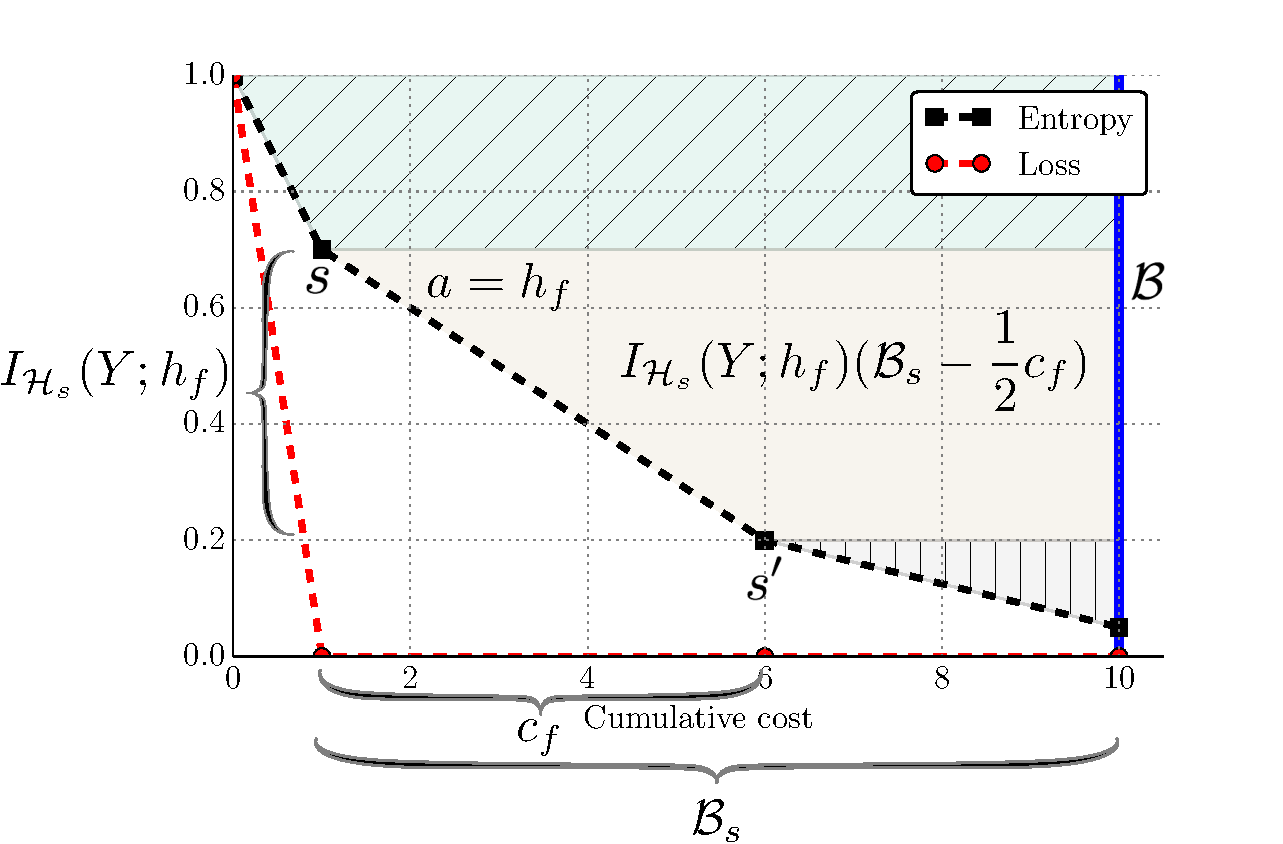
\includegraphics[width=1\linewidth]{../../figures/rewards.pdf}
\caption{
Definition of the reward function.
To maximize the total area above the entropy vs. cost curve from $0$ to $\mathcal{B}$, we define the reward of an individual action as the area of the slice of the total area that it contributes.
From state $s$, action $a = h_f$ leads to state $s'$ with cost $c_f$.
The information gain is $I_{\mathcal{H}_s}(Y; h_f) = H(Y; \mathcal{H}_s) - H(Y; \mathcal{H}_s \cup {h_f})$.
\label{fig:rewards}}
\end{figure}

\begin{mydef} \label{def:problem}
\textbf{The test-time efficient multi-class classification problem} consists of

\begin{itemize}
\addtolength{\itemsep}{-.55\baselineskip}
\item
$N$ instances labeled with one of $K$ labels: ${\mathcal{D} = \{x_n \in \mathcal{X}, y_n \in \mathcal{Y} = \{1, \dots, K\}\}_{n=1}^N}$.

\item
$F$ features $\mathcal{H} = \{h_f : \mathcal{X} \mapsto \mathbb{R}^{d_f} \}_{f=1}^F$, with associated costs $c_f$.

\item Budget-sensitive loss $\mathcal{L}_\mathcal{B}$, composed of cost budget $\mathcal{B}$ and loss function ${\ell(\hat{y}, y) \mapsto \mathbb{R}}$.
\end{itemize}

The goal is to find a \textbf{feature selection} policy $\pi(x): \mathcal{X} \mapsto 2^\mathcal{H}$ and a \textbf{feature combination} classifier $g(\mathcal{H}_\pi) : 2^\mathcal{H} \mapsto \mathcal{Y}$ such that such that the total budget-sensitive loss $\sum \mathcal{L}_\mathcal{B}(g(\pi(x_n)), y_n)$ is minimized.
\end{mydef}

%The features $h_f$ can be classifier outputs, possibly multi-class; following convention, we refer to such features as \emph{weak learners}.

The cost of a selected feature subset $\mathcal{H}_{\pi(x)}$ is $C_{\mathcal{H}_\pi(x)}$.
The budget-sensitive loss $\mathcal{L}_\mathcal{B}$ presents a \textbf{hard budget constraint} by only accepting answers with $C_{\mathcal{H}} \leq \mathcal{B}$.
Additionally, $\mathcal{L}_\mathcal{B}$ can be \textbf{cost-sensitive}: answers given with less cost are more valuable than costlier answers.
The motivation for the latter property is \emph{Anytime} performance; we should be able to stop our algorithm's execution at any time and have the best possible answer.

Feature costs $c_f$ can be specified flexibly, with options including theoretical analysis, number of flops, wall clock runtime, total CPU time, or exact power expenditure.
We believe that a deployment in a modern datacenter is most likely to optimize for power expenditure.
In the absence of reliable ways to measure power, we use total CPU time to define the cost: if an operation is performed in parallel on multiple cores, its cost is considered to be the total cpu time on all cores.

% For a weak learner $h_f$, the cost $c_f$ is composed of the cost of an underlying feature extraction $\phi_{h_f}(x)$ and the cost of subsequent classification.
% Once $h_f$ is computed, its underlying feature $\phi$ is considered to be free for all other features $h_f'$ that share it, if any, such that $c_f' < c_f$.
% Note that in state-of-the-art object recognition systems, complex features and feature encodings are often followed by linear classifiers, and feature extraction cost dominates the total cost.

% \todo{REDO this:}
% A quick preview of an instance of the defined problem is in order.
% On the ImageNet dataset, we could define $h_f$ as intersections of feature channels and class subsets:\\
% {\footnotesize\texttt{
% GIST.Animal, SIFT-BOW.Animal, LLC-SIFT.Animal,\\
% GIST.Vehicle, SIFT-BOW.Vehicle, LLC-SIFT.Vehicle.}}\\
% $\mathcal{G}$ could be defined by a hierarchical loss (accuracy at the leaf nodes counts more than accuracy at inner nodes), and $\mathcal{B}$ could only admit answers that take less than 5 seconds.

At training time, our computation is unbudgeted, and we can compute all features to have \emph{fully-observed} training instances.
At test time, there is a budget and so the instances we classify will only be \emph{partially-observed}, as determined by the feature selection policy.

We defer discussion of learning the \textbf{feature combination} classifier $g(\mathcal{H}_\pi) : 2^\mathcal{H} \mapsto \mathcal{Y}$ to~\autoref{sec:classifier}.
For now, we assume that $g$ can combine an arbitrary subset of features and provide a distribution $P(Y = y)$.
For example, $g$ could be a Naive Bayes (NB) model trained on the fully-observed data.

% \subsection{Static greedy selection.}
% Our initial goal is select a feature subset $\pi(x)$ such that $C_{\pi(x)} \leq \mathcal{B}$ and $\sum \ell(g(\pi(x_n)), y_n)$ is minimized.
% We assume that given a feature subset $\pi(x)$, we are able to find a classifier function $g$ such that the loss is minimized.

% If the classifier $g$ can give a full distribution $P(Y = y)$ and not just a prediction $y \in \{1, \dots, K\}$, we can maximize information gain of the selected subset, instead of directly minimizing the loss of $g(\pi(x))$:\[
% I(Y; \pi(x)) = H(Y) - H(Y | \pi(x)) = \sum_{y \in Y} P(y) \log P(y) -  \sum_{\substack{y \in Y,\\z \in Z}} P(y, z) \log P(y \mid z)
% \]
% To the extent that $g$ is unbiased, maximizing information gain corresponds to minimizing loss, and has the benefit of ensuring that we not only make the right classification decision but also become maximally certain.

% Finding the optimal subset is NP-hard.
% A common heuristic is simple greedy selection, which is known to be near-optimal for optimizing submodular set functions with unit-cost elements \parencite{Nemhauser-1978}.
% In case of non-uniform additive costs, it can be proven that when all features $h$ are independent given $Y$ (as in an NB classifier), building $\pi(x)$ by repeatedly selecting
% \begin{align*}
% h* = \argmax_{h \in \mathcal{H} \setminus \pi(x)} \frac{1}{c_f} \left[ H(h \mid \pi(x)) - H(h \mid Y) \right]
% \end{align*}
% while $C_{\pi(x)} \leq \mathcal{B}$ gives $I(Y; \pi(x)) \geq \frac{1}{2} (1 - 1/e) I_{\text{OPT}}$ with additional terms if the entropy calculation is not exact \parencite{Krause-UAI-2005}\footnote{A tighter (by factor of 2) bound is possible with a $O(F^5)$ instead of this $O(F^2)$ algorithm \parencite{Krause-note-2005}.}.

% However, we may find the feature independence assumption too restrictive or may not be able to reliably compute entropy.
% Additional difficulties come from introducing a setup cost or non-additive costs \todo{although we could resolve them.}
% When we make the feature selection dynamic---guided by the feature values observed---we will face further challenges if the structure of the problem necessitates a non-myopic solution.
% \todo{Need stronger explanation for why we are not proceeding with adaptive submodularity---or just not mention submodularity at all?}

\subsection{Dynamic feature selection as a Markov-Decision-Process (MDP).}
To model the \textbf{feature selection} policy $\pi(x): \mathcal{X} \mapsto 2^\mathcal{H}$, we introduce the Markov Decision Process (MDP), which defines a single \emph{episode} of selecting features for some instance $x$.

\begin{mydef} \label{def:MDP}
The \textbf{feature selection MDP} consists of the tuple $(\mathcal{S}, \mathcal{A}, T(\cdot), R(\cdot), \gamma)$:

\begin{itemize}\addtolength{\itemsep}{-.55\baselineskip}
\item \textbf{State} $s \in \mathcal{S}$ stores the selected feature subset $\mathcal{H}_{\pi(x)}$ and their values and total cost $C_{\mathcal{H}_{\pi(x)}}$.
\item The set of \textbf{actions} $\mathcal{A}$ is exactly the set of features $\mathcal{H}$.
\item The (stochastic) \textbf{state transition} distribution $T(s' \mid s, a)$ can depend on the instance $x$.
\item The \textbf{reward} function $R(s, a, s') \mapsto \mathbb{R}$ is manually specified, and depends on the classifier $g$ and the instance $x$.
\item The discount $\gamma$ determines amount of \textbf{lookahead} in selecting actions: if 0, actions are selected greedily based on their immediate reward; if 1, the reward accrued by subsequent actions is given just as much weight as the reward of the current action.
\end{itemize}
\end{mydef}

Running the MDP on a given instance $x$ gives a trajectory $\xi = (s_0, a_0, s_1, r_1, \dots, a_{I-1}, s_I, r_I)$, where $I$ is the total number of actions taken (and therefore features selected), $s_0$ is the initial state, $a_i \sim \pi(a \mid s_i)$ is chosen by the \emph{policy} $\pi(a \mid s)$, and $s_{i+1} \sim T(s \mid s_i, a_i)$, which can depend on $x$.
The total expected reward (value) of an MDP episode is written as
\begin{equation} \label{eq:expected_reward}
V_\pi(s_0) =
\mathbb{E}_{\xi \sim \left\{ \pi, x \right\}} r(\xi) =
\mathbb{E}_{\xi \sim \left\{ \pi, x \right\}} \left[ \sum_{i=0}^I \gamma^i \, r_i \right]
\end{equation}
Gathering such trajectories forms the basis of our policy learning method.

\subsection{Defining the reward.}
The budget-sensitive loss $\mathcal{L}_\mathcal{B}$ enforces \emph{Anytime} performance by valuing early gains more than later gains.
To formalize this, consider \hyperref[fig:rewards]{Figure~\ref*{fig:rewards}}, which shows the entropy and the 0-1 loss of $g$ at every point in a sequential feature selection episode for some instance $x$.
For the best \emph{Anytime} performance, we want to capture the most area above the loss vs. cost curve, up to max budget $\mathcal{B}$ \parencite{Karayev-NIPS-2012}.

Recall from \eqref{eq:expected_reward} that the value of an episode $\xi$ is defined as the sum of obtained rewards.
If the reward of a single action is defined as the area above the curve that is captured as a direct result, then the value of the whole episode exactly corresponds to $\mathcal{L}_\mathcal{B}$.

However, there is a problem with using loss directly: only the first action to ``tip the scale'' toward the correct prediction gets a direct reward (in the figure, it is the first action).  A smoother reward function is desirable:
if the classifier $g$ can give a full distribution $P(Y = y \mid \mathcal{H}_{\pi(x)})$ and not just a prediction $\hat{y} \in \mathcal{Y}$, we can maximize the \emph{information gain} of the selected subset instead of directly minimizing the loss of $g(\pi(x))$:
\begin{eqnarray}
I(Y; \mathcal{H}_{\pi(x)}) &=& H(Y) - H(Y | \mathcal{H}_{\pi(x)}) = \\ \notag
&=& \sum_{y \in Y} P(y) \log P(y) -  \\ \notag
&&\sum_{y, \mathcal{H}_{\pi(x)}} P(y, \mathcal{H}_{\pi(x)}) \log P(y \mid \mathcal{H}_{\pi(x)})
\end{eqnarray}
To the extent that $g$ is unbiased, maximizing information gain corresponds to minimizing loss, and ensures that we not only make the right classification decision but also become maximally certain.
Therefore, as graphically presented in \hyperref[fig:rewards]{Figure~\ref*{fig:rewards}}, we define the reward of selecting feature $h_s$ with cost $c_f$ with the set $\mathcal{H}_s$ computed to be $I_{\mathcal{H}_s}(Y; h_f) (\mathcal{B}_s - \frac{1}{2}c_f)$.

Although we do not evaluate in this regime, note that this definition easily incorporates a \textbf{setup cost} in addition to \textbf{deadline cost} by only computing the area in between setup and deadline costs.

\subsection{Parametrizing and learning the policy.}
% From the trajectories we can compute the \emph{value function} for any state:
% \begin{equation} \label{eq:value_function}
% V_\pi(s) = \sum_{s'} T_\pi(s, s') \left[ R_\pi(s, s') + \gamma V_\pi(s') \right]
% \end{equation}

Space constraints prohibit a full exposition of reinforcement learning techniques; \parencite{Sutton1998} provides a thorough review.
In brief: we seek $\pi$ that maximizes the expected value of the MDP \eqref{eq:expected_reward}.
Therefore, actions must be selected according to their expected \emph{value}:
\begin{align*}
\argmax_a \pi(a \mid s) = \argmax_a Q^*(s,a)
\end{align*}
where $Q^*(s,a)$ is the optimal \emph{action-value function}---the expected value of taking action $a$ in state $s$ and then acting optimally to the end of the episode.

Because the state represents an exponential number of subsets and associated real values, we cannot represent $Q(s,a)$ exactly.
Instead, we use feature approximation and write $Q(s,a) = \theta^T \phi(s, a)$,  where $\phi: \mathcal{S} \times \mathcal{A} \mapsto \mathbb{R}^{d_s}$ is the state featurization function, $d_s$ is the dimensionality of the state feature vector, and $\theta$ is a vector of weights that defines the policy.

Specifically, the policy is defined as
\begin{equation}
\pi(a \mid s) = \frac{1}{Z} \exp\left(\frac{1}{\tau} \theta^T \phi(s, a)\right)
\end{equation}
where $Z$ is the appropriate normalization and $\tau$ is a temperature parameter that controls the level of exploration vs. exploitation in the policy.
As $\tau \rightarrow 0$, ${\pi(a \mid s)}$ becomes highly peaked at $\argmax_a Q(s,a)$; it becomes uniform as $\tau \rightarrow \infty$.

As commonly done, we learn the $\theta$ by \emph{policy iteration}.
First, we gather $(s, a, r, s')$ samples by running episodes (to completion) with the current policy parameters $\theta_i$.
From these samples, $\hat{Q}(s, a)$ values are computed, and $\theta_{i+1}$ are given by $L_2$-regularized least squares solution to $\hat{Q}(s, a) = \theta^T \phi(s, a)$, on all states that we have seen in training.

During training, we gather samples starting from either a random feasible state, with probability $\epsilon$, or from the initial empty state otherwise.
Both $\epsilon$ and $\tau$ parameters decay exponentially with the number of training iterations.
Training is terminated if $\pi_{\theta_{i+1}}$ returns the exact same sequence of episodes $\xi$ on a validation set as $\pi_{\theta_{i}}$.

\paragraph{Static vs. Dynamic state-action feature vector.}\label{sec:policy_features}
The featurization function $\phi(s)$ extracts the following features from the state:
\begin{itemize}\addtolength{\itemsep}{-.5\baselineskip}
\item Bit vector $\textbf{m}$ of length $F$: initially all bits are $1$ and are set to $0$ when the corresponding feature is computed.
\item For each $h_f$, a vector of size $d_f$ representing the values; $0$ until observed.
\item Cost feature $c \in [0, 1]$, for fraction of the budget spent.
\item Bias feature $1$.
\end{itemize}

\begin{algorithm}[]
\SetKwFunction{ComputeRewards}{ComputeRewards}
\SetKwFunction{GatherSamples}{GatherSamples}
\SetKwFunction{UpdatePolicy}{UpdatePolicy}
\SetKwFunction{UpdateClassifier}{UpdateClassifier}

\SetAlgoLined
\KwIn{$\mathcal{D} = \{x_n, y_n\}_{n=1}^N$; $\mathcal{L}_\mathcal{B}$}
\KwResult{Trained $\pi$, $g$}
\BlankLine
$\pi_0 \leftarrow$ random\;
\For {$i \leftarrow 1$ \KwTo max\_iterations} {
    States, Actions, Costs, Labels $\leftarrow$ \GatherSamples{$\mathcal{D}$, $\pi_{i-1}$}\;
    $g_i \leftarrow$ \UpdateClassifier{States, Labels}\;
    Rewards $\leftarrow$ \ComputeRewards{States, Costs, Labels, $g_i, \mathcal{L}_\mathcal{B}, \gamma$}\;
    $\pi_i \leftarrow$ \UpdatePolicy{States, Actions, Rewards}\;
}
\caption{Because reward computation depends on the classifier, and the distribution of states depends on the policy, $g$ and $\pi$ are trained iteratively.\label{alg:learning}}
\end{algorithm}

These features define the \textbf{dynamic} state, presenting enough information to have a \emph{closed-loop} (dynamic) policy that may select different features for different test instances.
The \textbf{static} state has all of the above features except for the observed feature values.
This enables only an \emph{open-loop} (static) policy, which is exactly the same for all instances.
Policy learned with the static state is used as a baseline in experiments.

The state-action feature function $\phi(s, a)$ effectively block-codes these features: it is $0$ everywhere except the block corresponding to the action considered.
In implementation, we train $F$ separate regressions with a tied regularization parameter, which is K-fold cross-validated.

\paragraph{Effect of $\gamma$.}
Note that solving the MDP with these features and with $\gamma=0$ finds a \textbf{Static, greedy} policy: the value of taking an action in a state is exactly the expected reward to be obtained.
When $\gamma=1$, the value of taking an action is the entire area above the curve as defined in \autoref{fig:rewards}, and we learn the \textbf{Static, non-myopic} policy---another baseline.

\subsection{Learning the classifier.}\label{sec:classifier}

We have so far assumed that $g$ can combine an arbitrary subset of features and provide a distribution $P(Y = y)$---for example, a Gaussian Naive Bayes (NB) model trained on the fully-observed data.
% However, a Naive Bayes classifier suffers from its restrictive independence assumptions.

Since discriminative classifiers commonly provide better performance, we use a \textbf{logistic regression} classifier, which presents a new challenge:
% bu have to account for missing data:
at test time, some feature values are missing and need to be imputed.
If the classifier is trained exclusively on fully-observed data, then the feature value statistics at test time will not match, resulting in poor performance.
Therefore, we need to learn classifier weights on a distribution of data that exhibits the pattern of missing features induces by the policy $\pi$.
At the same time, learning the policy depends on the classifier $g$, used in the computation of the rewards.
For this reason, the policy and classifier need to be learned jointly: \autoref{alg:learning} gives the iterative procedure.

\paragraph{Unobserved value imputation.}
Unlike the Naive Bayes classifier, the logistic regression classifier is not able to use an arbitrary subset of features $\mathcal{H}_\pi$, but instead operates on feature vectors of a fixed size.
To represent the feature vector of a fully observed instance, we write $\mathbf{x} = [h_1(x), \dots, h_f(x)]$.
In case that $\mathcal{H}_\pi \subset \mathcal{H}$, we need to fill in unobserved feature values in the vector.

A basic strategy is \textbf{mean imputation}: filling in with the mean value of the feature:
\begin{align}
\mathbf{x}_\pi = \left[ h_i(x) : \left\{ \begin{array}{rl}
 h_i(x) &\mbox{ if $h_i \in \mathcal{H}_{\pi(x)}$} \\
 \bar{\mathbf{h}}_i &\mbox{ otherwise}
\end{array} \right. \right]
\end{align}

If we assume that $\mathbf{x}$ is distributed according to a multivariate Gaussian $\mathbf{x} \sim \mathcal{N}(\mathbf{0}, \Sigma)$, where $\Sigma$ is the sample covariance $X^T X$ and the data is standardized to have zero mean, then it is possible to do \textbf{Gaussian imputation}.
Given a feature subset $\mathcal{H}_\pi$, we write:
\begin{equation}
\mathbf{x}_\pi = \begin{bmatrix} \mathbf{x}^\text{o}\\  \mathbf{x}^\text{u} \end{bmatrix} \sim \mathcal{N} \left( \mathbf{0}, \begin{bmatrix} \mathbf{A} & \mathbf{C}\\ \mathbf{C}^T & \mathbf{B} \end{bmatrix} \right)
\end{equation}
where $\mathbf{x}^\text{o}$ and $\mathbf{x}^\text{u}$ represent the respectively observed and unobserved parts of the full feature vector $\mathbf{x}$.
%, $\mathbf{A}$ is the covariance matrix of $\mathbf{x}^\text{o}$, $\mathbf{B}$ is the covariance matrix of $\mathbf{x}^\text{u}$, and $C$ is the cross-variance matrix that has as many rows as the size of $\mathbf{x}^\text{o}$ and as many columns as the size of $\mathbf{x}^\text{u}$.
%\parencite{Roweis-gaussian-identities}.
In this case, the distribution over unobserved variables conditioned on the observed variables is given as
$\mathbf{x}^\text{u} \mid \mathbf{x}^\text{o} \sim \mathcal{N} \left( \mathbf{C}^T \mathbf{A}^{-1} \mathbf{x}^\text{o},\, \mathbf{B} - \mathbf{C}^T \mathbf{A}^{-1} \mathbf{C} \right)$.

\paragraph{Learning more than one classifier.}
As illustrated in \hyperref[fig:state_space]{Figure~\ref*{fig:state_space}}, the policy $\pi$ selects some feature subsets more frequently than others.
Instead of learning only one classifier $g$ that must be robust to all observed feature subsets, we can learn several classifiers, one for each of the most frequent subsets.
This is done by maintaining a distribution over encountered feature subsets during training.
For each of the $K$ most frequent subsets, a separate classifier is trained, using data that is closest by Hamming distance on the selected-feature bit vector.

Each classifier is trained with the \textsc{Liblinear} implementation of logistic regression, with $L_2$ regularization parameter K-fold cross-validated at each iteration.

\begin{figure}[ht]
\centering
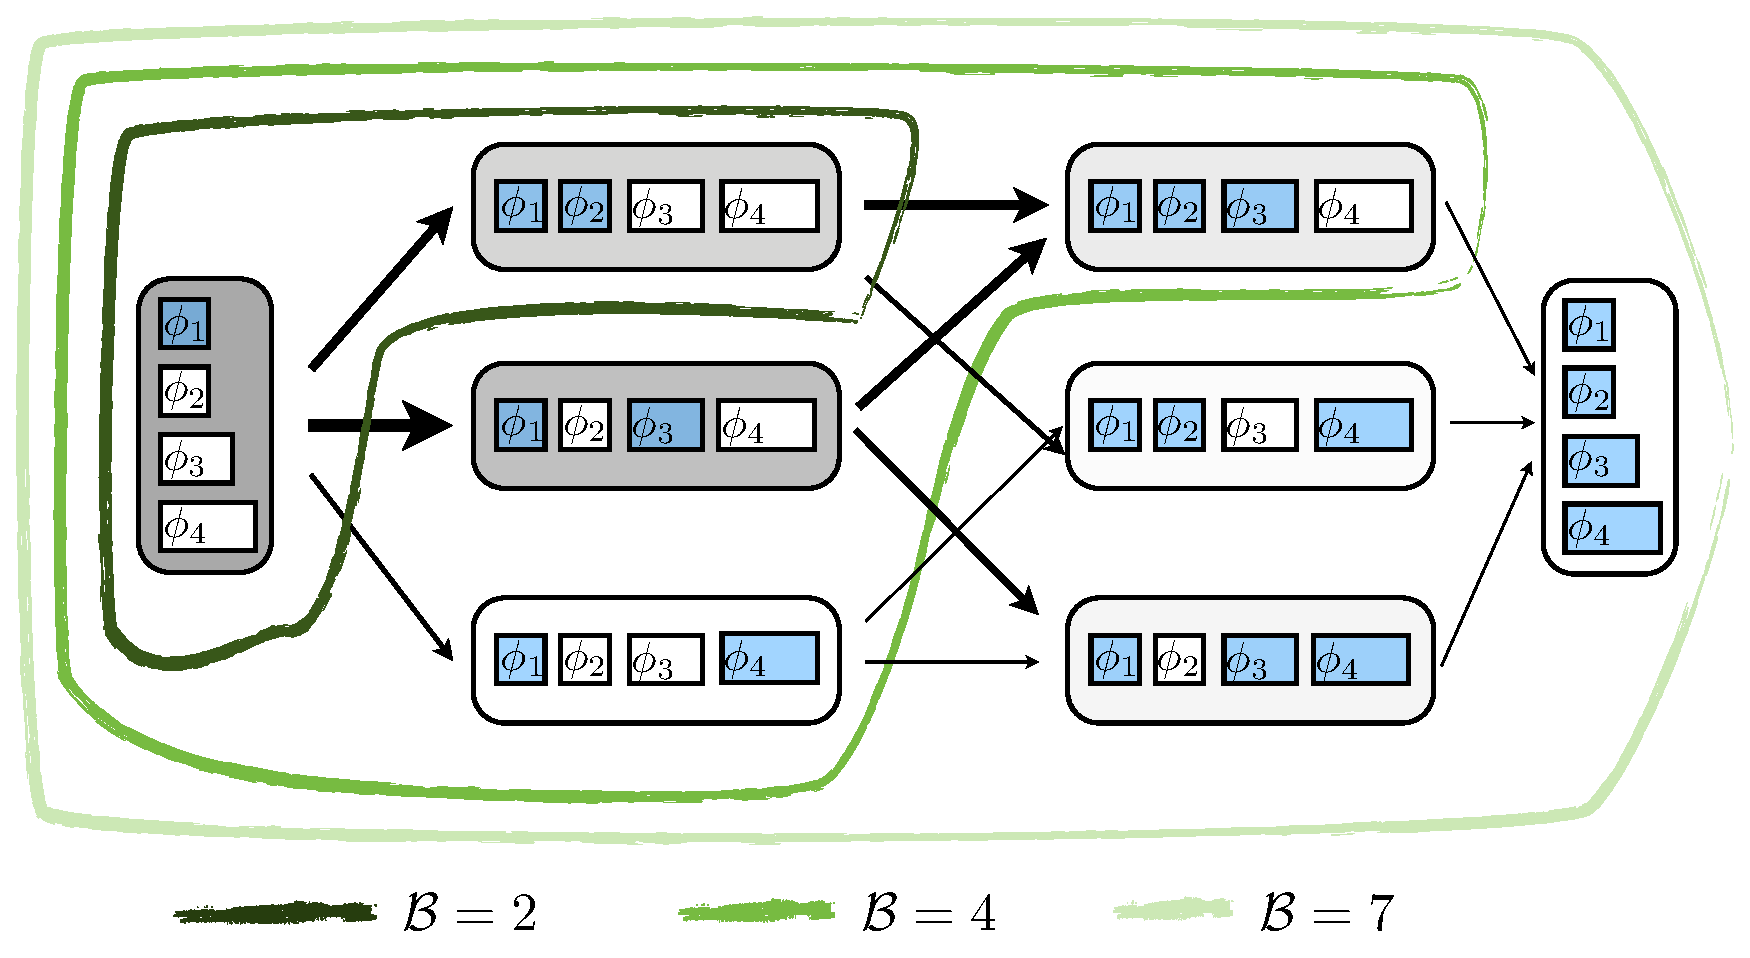
\includegraphics[width=1\linewidth]{../../figures/mdp_masks.pdf}
\caption{
The action space $\mathcal{A}$ of the MDP is the the set of features $\mathcal{H}$, represented by the $\phi$ boxes.
The primary discretization of the state space can be visualized by the possible feature subsets (larger boxes); selected features are colored in the diagram.
The feature selection policy $\pi$ induces a distribution over feature subsets, for a dataset, which is represented by the shading of the larger boxes.
Not all states are reachable for a given budget $\mathcal{B}$.
In the figure, we show three ``budget cuts'' of the state space.
\label{fig:state_space}
}
\end{figure}

\section{Evaluation}
We evaluate the following sequential selection baselines:
\begin{itemize}\addtolength{\itemsep}{-.35\baselineskip}
\item \textbf{Static, greedy}: corresponds to best performance of a policy that does not observe feature values and selects actions greedily ($\gamma=0$).
\item \textbf{Static, non-myopic}: policy that does not observe feature values but uses the MDP machinery with $\gamma=1$ to consider future action rewards.
\item \textbf{Dynamic, greedy}: policy that observed feature values, but selects actions greedily.
% \item \todo{
% \textbf{Active Classification} \parencite{Gao-NIPS-2011}:
% Feature selection is done by greedy selection based on expected information gain divided by cost (so reward is information gain, $\gamma=0$).
% The feature responses are modeled as a mixture of multivariate Gaussians (one mixture element per class label), and inference is instance-specific, akin to locally weighted regression.
% Feature combination is done by the same model: the posteriors are used as the final answers.
% }
% \item
% \todo{\textbf{MD-DAG} \parencite{Benbouzid-ICML-2012}
% Feature selection is done by an MDP policy with three actions: Skip, Evaluate, Quit over a pre-determined sequence of weak learners (unspecified exactly how the sequence is arranged, except ``by quality'').
% }
\end{itemize}
Our method is the \textbf{Dynamic, non-myopic} policy: observed feature values, and full lookahead.

% In addition to the settings above, we evaluate three additional baselines that do not do any selection at all: (a) \textbf{all} features computed; (b) only the \textbf{best} feature (in terms of $\mathcal{G}$) computed; (c) only the \textbf{least costly} feature computed.

In preliminary experiments, Logistic Regression always performed better than the Gaussian Naive Bayes classifier, and so only the former is used in the experiments below.
As described above, we evaluated classification with \textbf{Gaussian} vs. \textbf{Mean} imputation, and with different number of classifiers (1, 3, and 6) clustered by feature subsets.
We found that mean imputation performed better than Gaussian imputation, and although increased number of classifiers sometimes increased performance, it also made our method more prone to overfitting; $K=1$ classifiers worked best on all tasks.
%For reason of space, we report only the best achieved performance in the following evaluation results.

We evaluate two forms of test-time efficient performance measure: the area under the curve and the performance at max budget, although note that all methods are trained only for the former measure.

While the individual implementation details have been largely provided in the preceding text, here we additionally note that some of our policy and classifier implementations use the scikit-learn package \parencite{Pedregosa2011}.

% \subsection{Baselines}
% \paragraph{Active Classification \parencite{Gao-NIPS-2011}}
% Feature selection is done by greedy selection based on expected information gain divided by cost (so reward is information gain, $\gamma=0$).
% The feature responses are modeled as a mixture of multivariate Gaussians (one mixture element per class label), and inference is instance-specific, akin to locally weighted regression.
% Feature combination is done by the same model: the posteriors are used as the final answers.

% \paragraph{Greedy Miser \parencite{Xu-ICML-2012}}
% Feature selection is done by the CART algorithm \parencite{Breiman-1984} with an impurity function that considers feature cost.
% Feature combination is an ensemble of trees.

% \paragraph{MD-DAG \parencite{Benbouzid-2012-ICML}}
% Feature selection is done by an MDP policy with three actions: Skip, Evaluate, Quit over a pre-determined sequence of weak learners (unspecified exactly how the sequence is arranged, except ``by quality'').
% Feature combination is an unweighted sum.

% \paragraph{Timely \parencite{Karayev-NIPS-2012}}
% Feature selection is done by MDP trained using a state feature vector that has the inference output of an MRF combining feature values.
% Feature combination is done by the same MRF.

\begin{figure*}[ht]
\centering
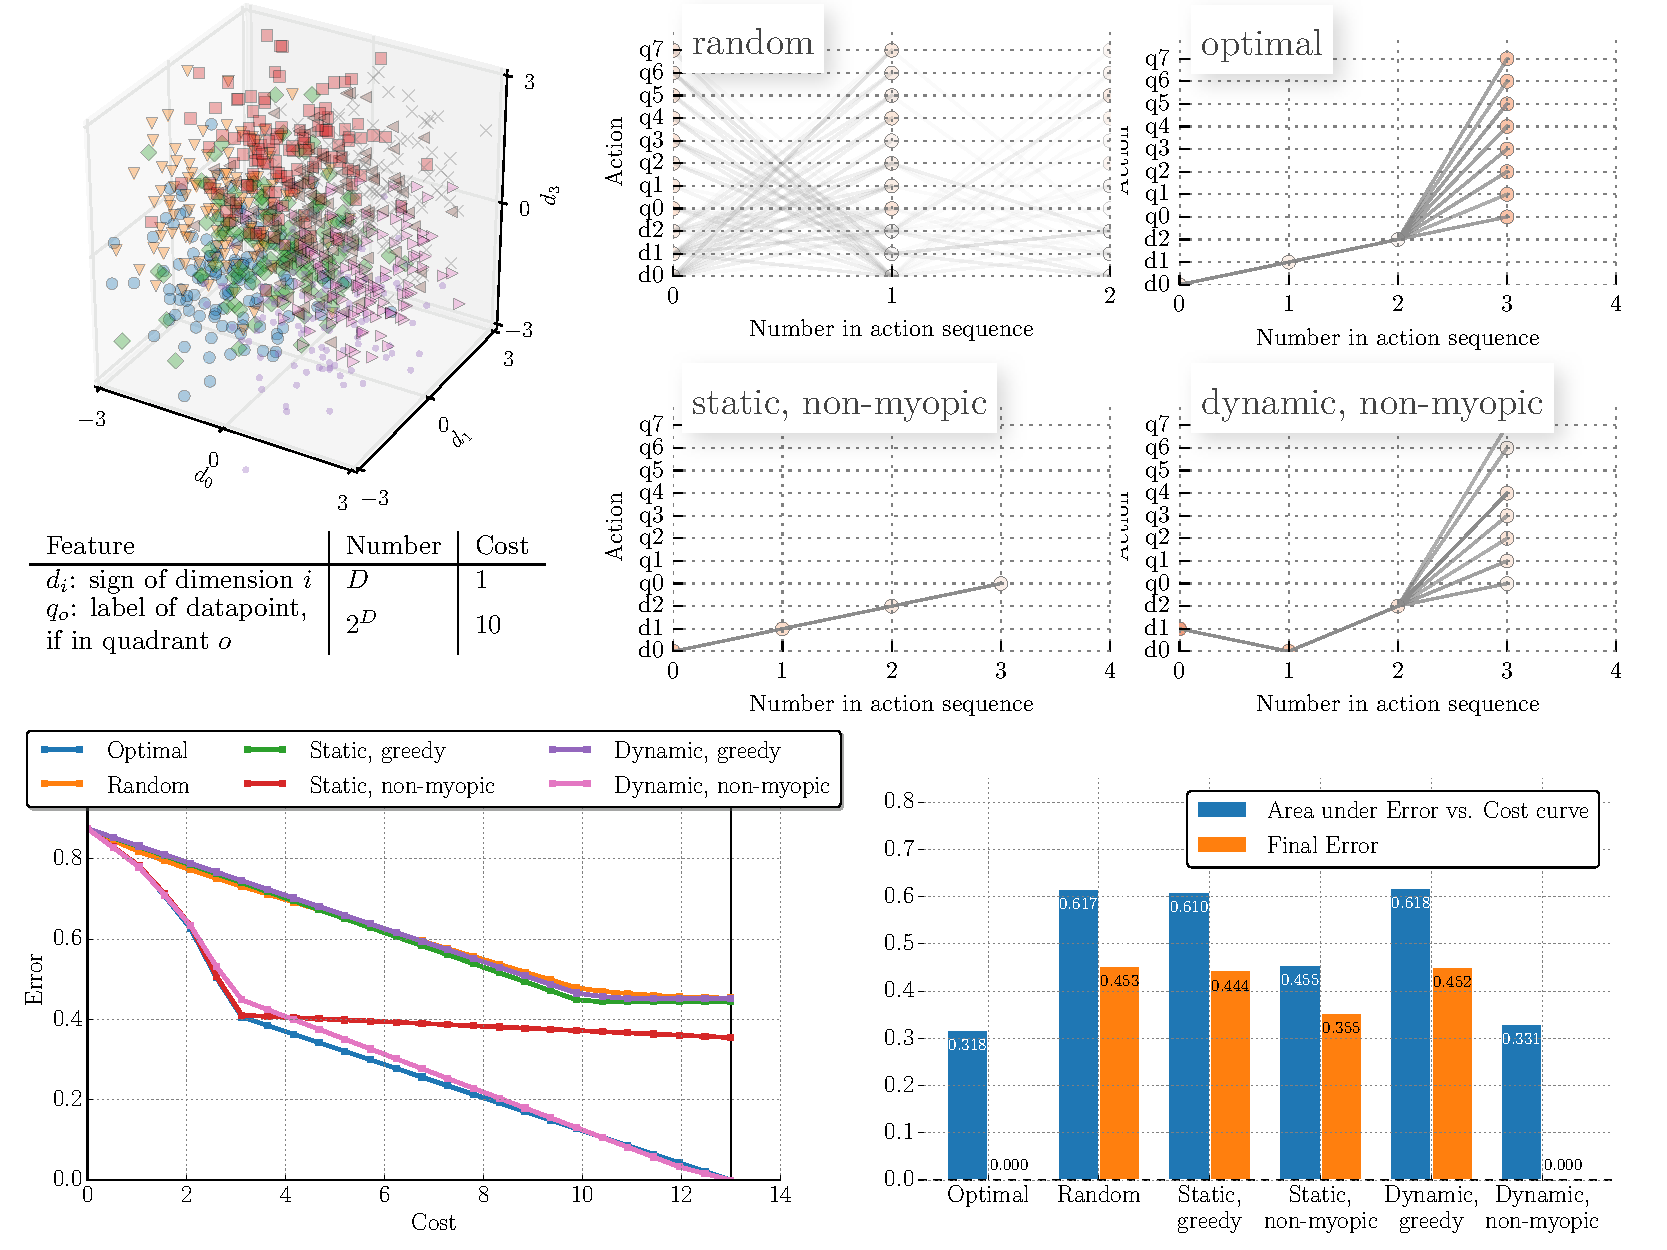
\includegraphics[width=.9\textwidth]{../../figures/synthetic.pdf}
\caption{
Evaluation on the synthetic example (best viewed in color).
The data and the feature costs are shown at top left; the sample feature trajectories of different policies at top right.
(The opacity of the edges corresponds to their prevalence during policy execution; the opacity of the nodes corresponds to the amount of reward obtained in that state.)
Note that the \emph{static, non-myopic} policy correctly learns to select the cheap features first, but is not able to correctly branch, while our \emph{dynamic, non-myopic} approach finds the optimal strategy.
The plots in the bottom half give the error vs. cost numbers.
}

\label{fig:synthetic}
\end{figure*}

\subsection{Synthetic Experiment.}
Following \parencite{Xu-ICML-2013}, we first show that the policy works as advertised in a challenging synthetic example.
In $D$-dimensional space, the data has a label for each of the $2^D$ orthants, and is generated by a unit-variance Gaussian in that orthant (See top left of \autoref{fig:synthetic} for the 3D case).
There are $D$ cheap features that simply return the sign of the data point's coordinate for the corresponding dimension.
For each orthant, there is also an expensive feature that returns the data point's label if the point is located in the corresponding orthant, and random noise otherwise.

The optimal policy on a new data point is to determine its orthant with cheap features, and then take the corresponding expensive action.
Note that both dynamic features and non-myopic learning are crucial to the optimal policy, which is successfully found by our approach.
\autoref{fig:synthetic} shows the results of this optimal policy, a random policy, and of different baselines and our method, trained given the correct minimal budget.

\subsection{Scene recognition.}
The Scene-15 dataset \parencite{Lazebnik-CVPR-2006} contains 4485 images from 15 visual scene classes.
The task is to classify images according to scene.
Following \parencite{Xiao-CVPR-2010}, we extracted 14 different visual features (GIST, HOG, TinyImages, LBP, SIFT, Line Histograms, Self-Similarity, Textons, Color Histograms, and variations).
The features vary in cost from 0.3 seconds to 8 seconds, and in single-feature accuracy from 0.32 (TinyImages) to .82 (HOG).
Separate multi-class linear SVMs were trained on each feature channel, using a random 100 positive example images per class for training.
We used the \texttt{liblinear} implementation, and K-fold cross-validated the penalty parameter $C$.
The trained SVMs were evaluated on the images not used for training, resulting in a dataset of 2238 vectors of 210 confidence values: 15 classes for each of the 14 feature channels.
This dataset was split 60-40 into training and test sets for our experiments.

\hyperref[fig:scenes]{Figure~\ref*{fig:scenes}} shows the results, including learned policy trajectories.
For all evaluated budgets, our \emph{dynamic, non-myopic} method outperforms all others on the area under the error vs. cost curve metric.
Our results on this dataset match the reported results of Active Classification \parencite{Gao-NIPS-2011} (Figure 2) and Greedy Miser \parencite{Xu-ICML-2012} (Figure 3), although both methods use an additional powerful feature channel (ObjectBank)\footnote{Detailed results for this and other experiments are on the project page (see front page for the \href{http://sergeykarayev.com/recognition-on-a-budget/}{link}).}.


\subsection{ImageNet and maximizing specificity.}
The full ImageNet dataset has over 10K categories and over a million images \parencite{Deng-ECCV-2010}.
The classes are organized in a hierarchical structure, which can be exploited for novel recognition tasks.
We evaluate on a 65-class subset introduced in ``Hedging Your Bets'' \parencite{Deng-CVPR-2012}.
In this evaluation, we consider the situation where the initial feature computation has already happened, and the task is to find a path through existing one-vs-all classifiers: features correspond to Platt-scaled SVM confidences of leaf-node classifiers (trained on SIFT-LLC features), and each has cost 1 \parencite{Deng-ECCV-2010}.
Following \parencite{Deng-CVPR-2012}, accuracy is defined on all nodes, and inner node confidences are obtained by summing the probabilities of the descendant nodes.

We combine our sequential feature selection with the ``Hedging Your Bets'' method for backing off prediction nodes using the ImageNet hierarchy to maintain guaranteed accuracy while giving maximally specific answers, given a cost budget.
The results are given in \hyperref[fig:imagenet]{Figure~\ref*{fig:imagenet}}.
As the available budget increases, the \emph{specificity} (defined by normalized information gain in the hierarchy) of our predictions also increases, while accuracy remains constant.
Visualizing this on the ILSVRC-65 hierarchy, we see that the fraction of predictions at the leaf nodes grows with available computation time.
This formulation presents a novel angle on modeling the time course of human visual perception.

\begin{figure*}[ht]
\centering
    \centering
    \begin{subfigure}[b]{0.39\textwidth}
            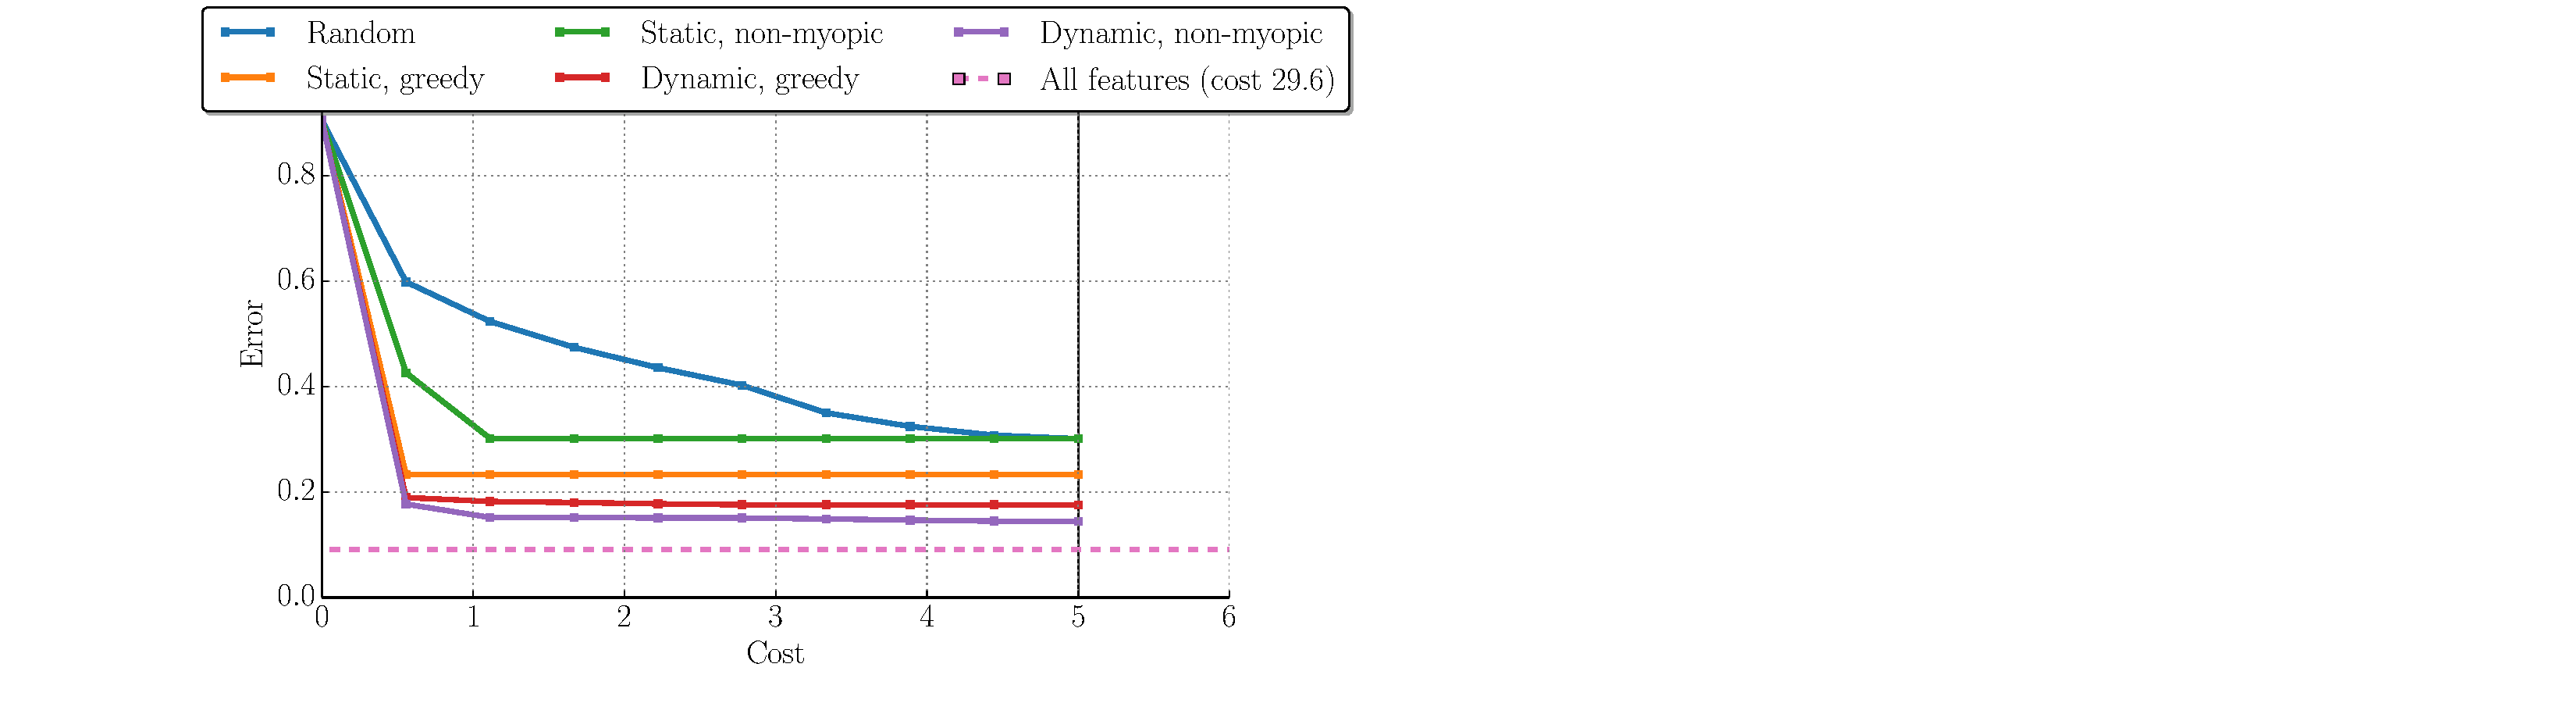
\includegraphics[width=\textwidth]{../../figures/apr11_assembly/scene_15_5_crop.pdf}
            \caption{Error given by policies learned for a budget = 5.}
    \end{subfigure}%
    \begin{subfigure}[b]{0.36\textwidth}
            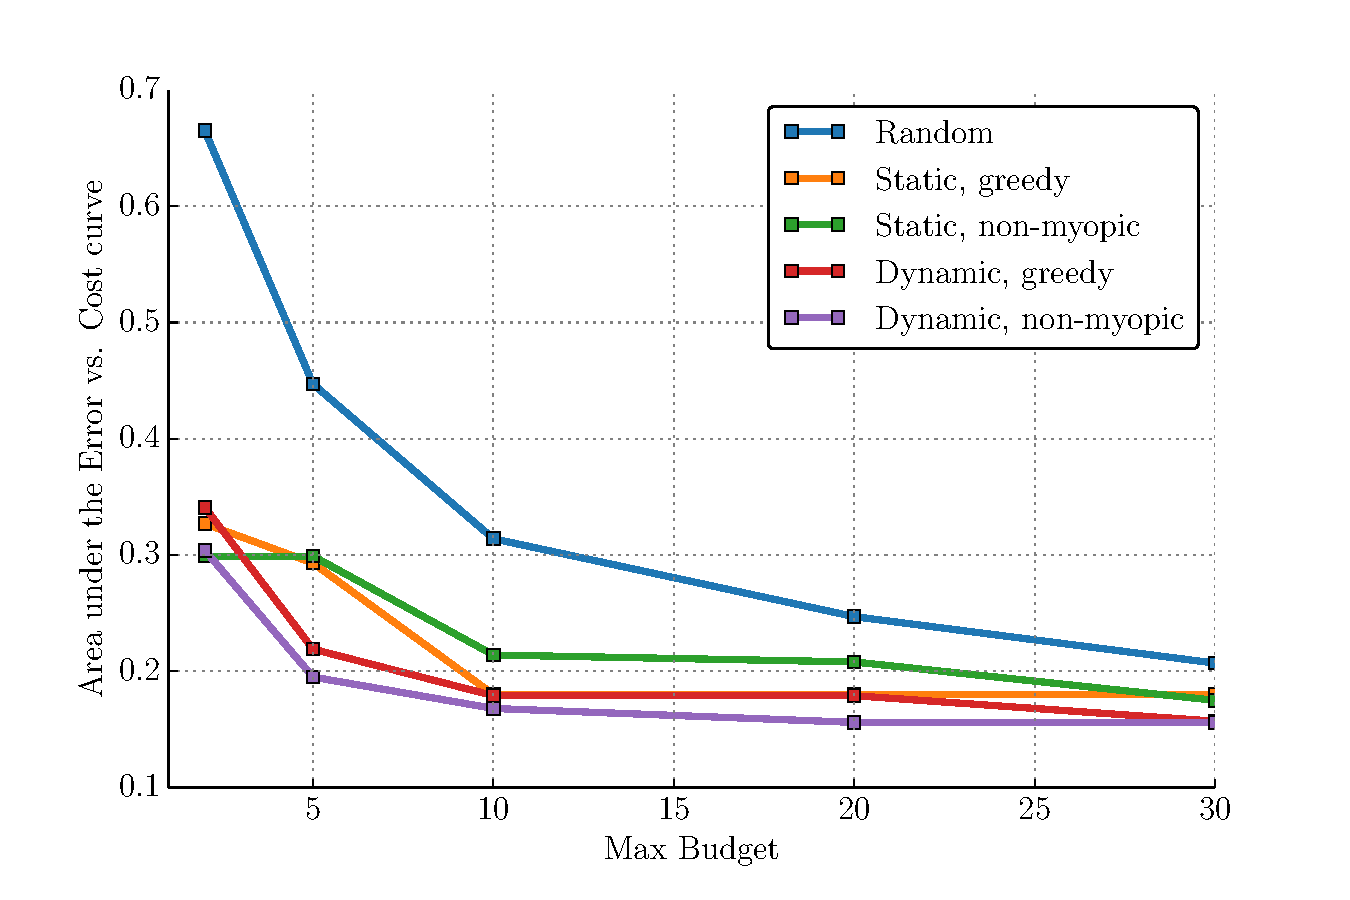
\includegraphics[width=\textwidth]{../../figures/apr11_assembly/_scenes15_auc.pdf}
            \caption{Areas under error vs. cost curves of policies learned at different budgets.}
    \end{subfigure}%
    \begin{subfigure}[b]{0.25\textwidth}
            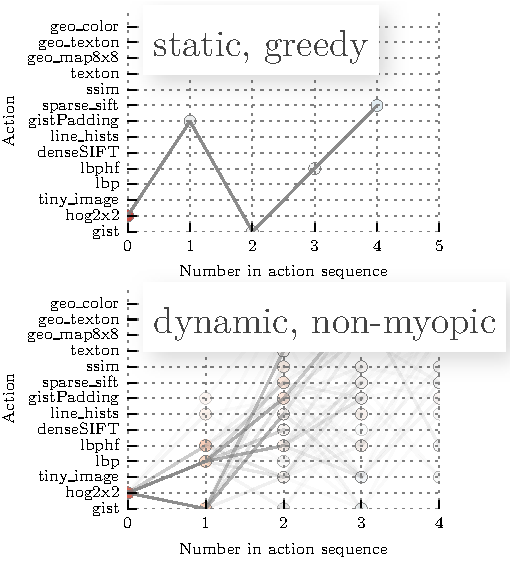
\includegraphics[width=\textwidth]{../../figures/apr11_assembly/scenes_result.pdf}
            \caption{Policy trajectories.}
    \end{subfigure}

    \caption{
Results on Scenes-15 dataset (best viewed in color).
Figure (a) shows the error vs. cost plot for policies learned given a budget of 5 seconds.
Figure (b) aggregates the area under the error vs. cost plot metrics for different policies and budgets, showeing that our approach outperforms baselines no matter what budget it's trained for.
Figure (c) shows the branching behavior of our dynamic policy.
\label{fig:scenes}
    }
\end{figure*}
\begin{figure*}[ht]
\centering
    \begin{subfigure}[b]{0.52\textwidth}
            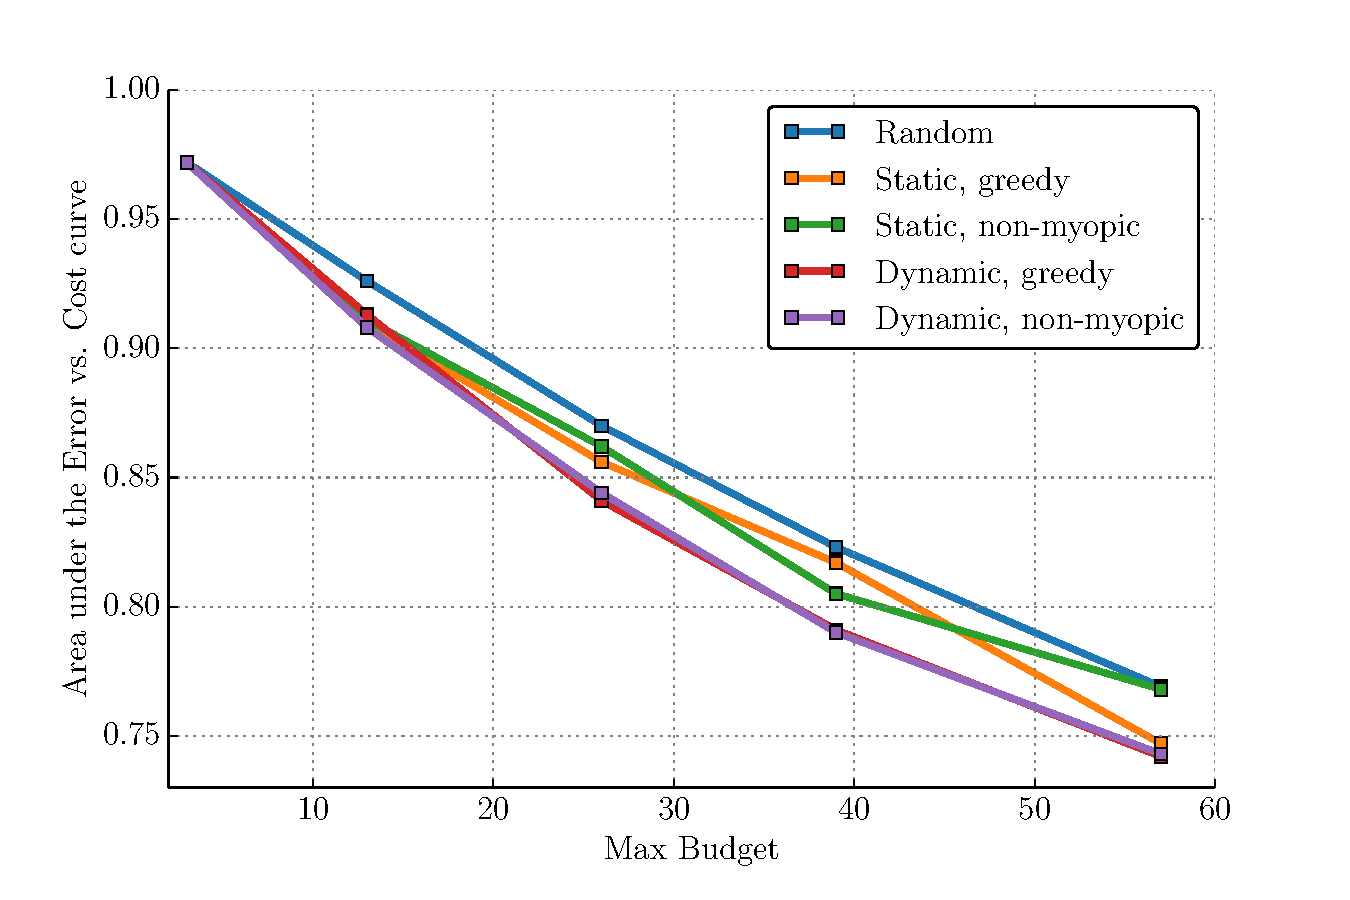
\includegraphics[width=\textwidth]{../../figures/apr11_assembly/_ilsvrc65_auc.pdf}
            \caption{
            Areas under error vs. cost curves for policies learned at different budgets.
            (No specificity back-off is performed here).
            \label{fig:imagenet-a}
            }
    \end{subfigure}\hfill%
    \begin{subfigure}[b]{0.43\textwidth}
            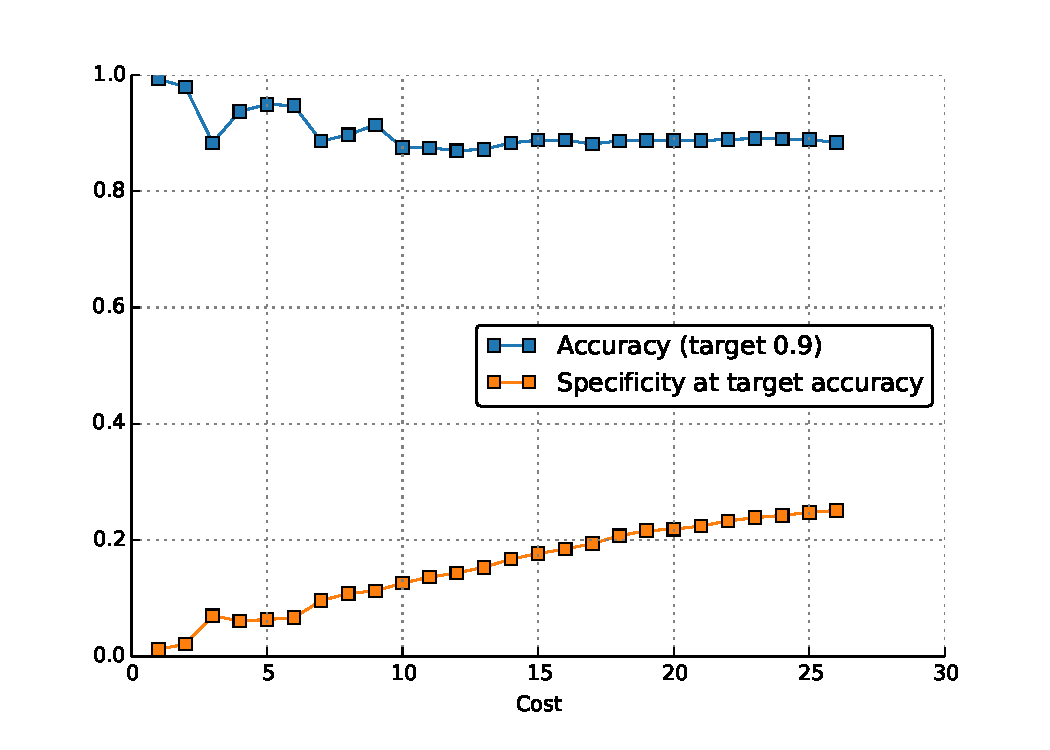
\includegraphics[width=\textwidth]{../../figures/apr11_assembly/ilsvrc65_acc.pdf}
            \caption{
            Holding prediction accuracy constant, we achieve increased specificity with increased cost (on \emph{Dynamic, non-myopic} policy, budget = 36).
            \label{fig:imagenet-b}
            }
    \end{subfigure}\\\vspace{1em}
    \begin{subfigure}[b]{.97\textwidth}
            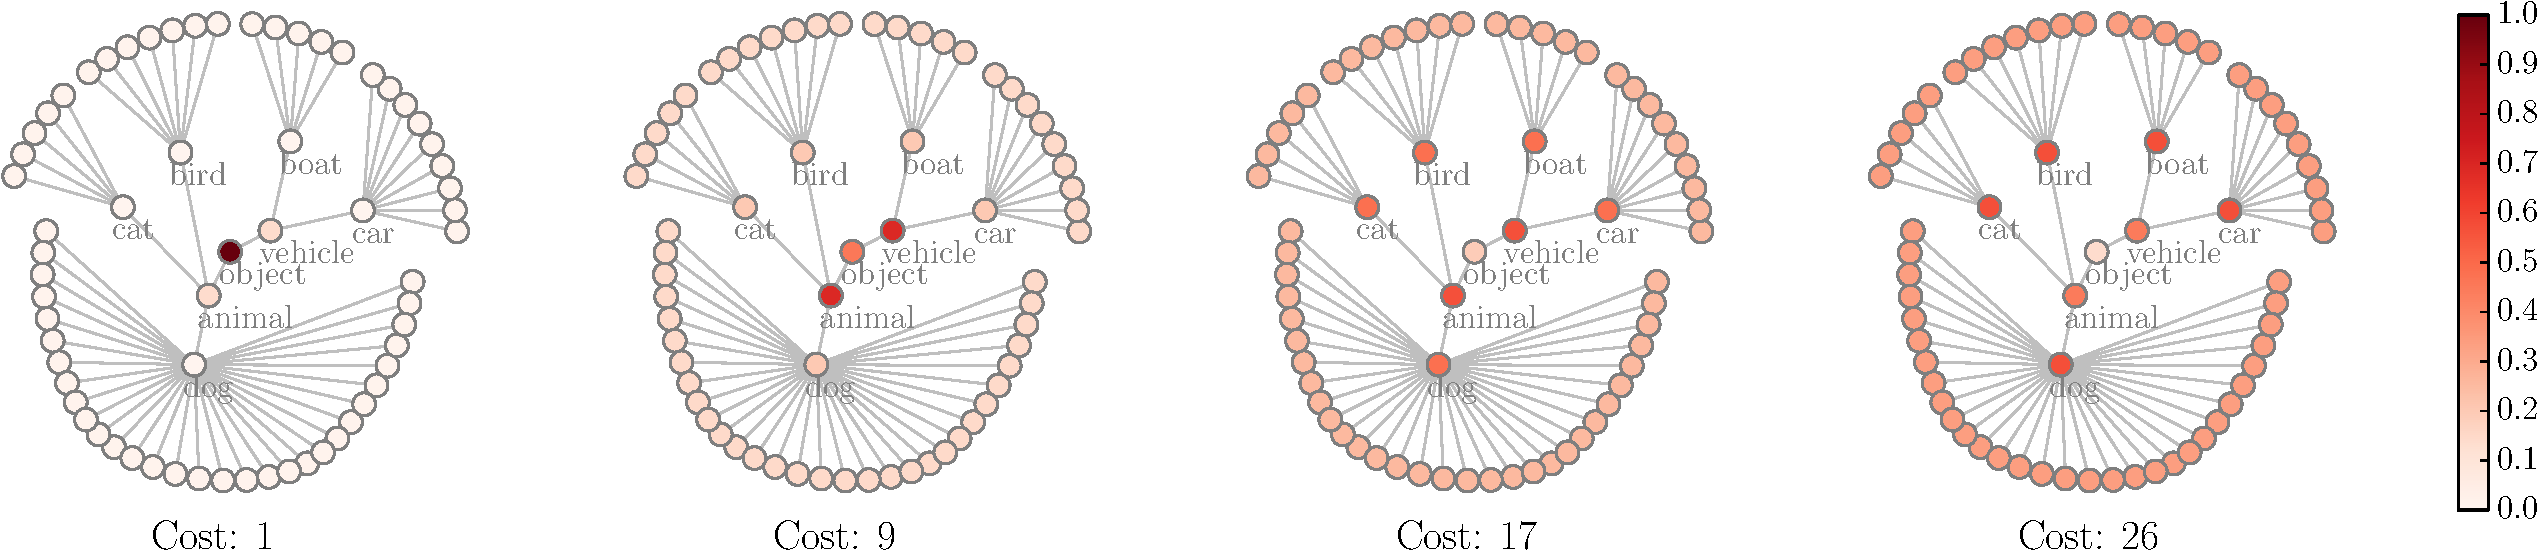
\includegraphics[width=\textwidth]{../../figures/apr11_assembly/ilsvrc65_network-crop.pdf}
            \caption{
            We visualize the fraction of predictions made at inner vs. leaf nodes of ILSVRC-65 at different cost points of an Anytime policy: with more computation, accurate predictions are increasingly made at the leaf nodes.
            \label{fig:imagenet-c}
            }
    \end{subfigure}

\caption{
Results on the ILSVRC-65 dataset (best viewed in color).
Figure (a) shows our dynamic approaches outperforming static baselines for all practical cost budgets.
When our method is combined with Hedging Your Bets \parencite{Deng-CVPR-2012}, a constant prediction accuracy can be achieved at all points in the Anytime policy, with \emph{specificity} of predictions increasing with the cost of predictions.
Figures (b) and (c) show this for the \emph{dynamic, non-myopic} policy learned for budget = 26.
This is analogous to human visual performance, which shows increased specificity at longer stimulus times.
\label{fig:imagenet}}
\end{figure*}

%!TEX root=../paper/thesis.tex
\chapter{Reinforcement Learning for Anytime Classification}

\section{Anytime Classification by Cost-sensitive Dynamic Feature Selection}

\begin{figure}[ht]
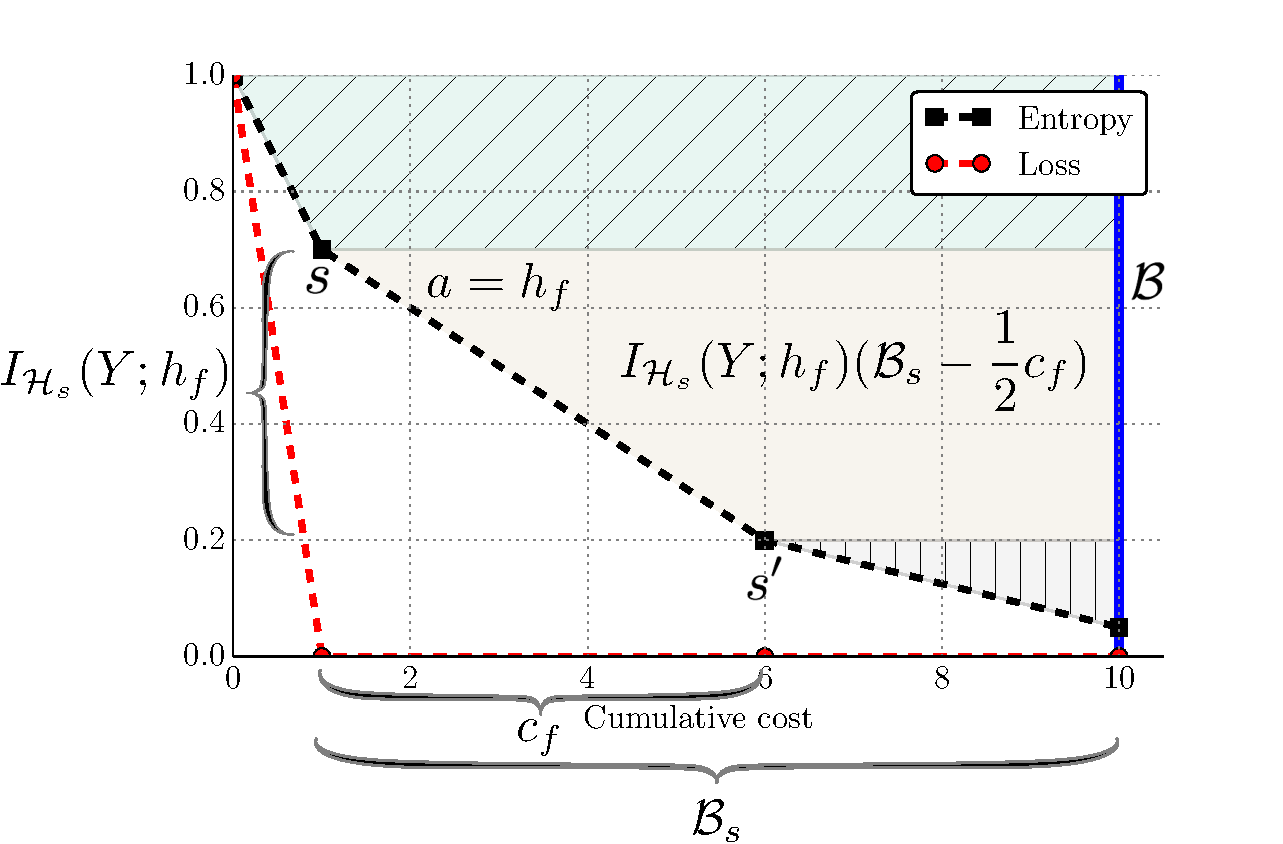
\includegraphics[width=1\linewidth]{../../figures/rewards.pdf}
\caption{
Definition of the reward function.
To maximize the total area above the entropy vs. cost curve from $0$ to $\mathcal{B}$, we define the reward of an individual action as the area of the slice of the total area that it contributes.
From state $s$, action $a = h_f$ leads to state $s'$ with cost $c_f$.
The information gain is $I_{\mathcal{H}_s}(Y; h_f) = H(Y; \mathcal{H}_s) - H(Y; \mathcal{H}_s \cup {h_f})$.
\label{fig:rewards}}
\end{figure}

\begin{mydef} \label{def:problem}
\textbf{The test-time efficient multi-class classification problem} consists of

\begin{itemize}
\addtolength{\itemsep}{-.55\baselineskip}
\item
$N$ instances labeled with one of $K$ labels: ${\mathcal{D} = \{x_n \in \mathcal{X}, y_n \in \mathcal{Y} = \{1, \dots, K\}\}_{n=1}^N}$.

\item
$F$ features $\mathcal{H} = \{h_f : \mathcal{X} \mapsto \mathbb{R}^{d_f} \}_{f=1}^F$, with associated costs $c_f$.

\item Budget-sensitive loss $\mathcal{L}_\mathcal{B}$, composed of cost budget $\mathcal{B}$ and loss function ${\ell(\hat{y}, y) \mapsto \mathbb{R}}$.
\end{itemize}

The goal is to find a \textbf{feature selection} policy $\pi(x): \mathcal{X} \mapsto 2^\mathcal{H}$ and a \textbf{feature combination} classifier $g(\mathcal{H}_\pi) : 2^\mathcal{H} \mapsto \mathcal{Y}$ such that such that the total budget-sensitive loss $\sum \mathcal{L}_\mathcal{B}(g(\pi(x_n)), y_n)$ is minimized.
\end{mydef}

%The features $h_f$ can be classifier outputs, possibly multi-class; following convention, we refer to such features as \emph{weak learners}.

The cost of a selected feature subset $\mathcal{H}_{\pi(x)}$ is $C_{\mathcal{H}_\pi(x)}$.
The budget-sensitive loss $\mathcal{L}_\mathcal{B}$ presents a \textbf{hard budget constraint} by only accepting answers with $C_{\mathcal{H}} \leq \mathcal{B}$.
Additionally, $\mathcal{L}_\mathcal{B}$ can be \textbf{cost-sensitive}: answers given with less cost are more valuable than costlier answers.
The motivation for the latter property is \emph{Anytime} performance; we should be able to stop our algorithm's execution at any time and have the best possible answer.

Feature costs $c_f$ can be specified flexibly, with options including theoretical analysis, number of flops, wall clock runtime, total CPU time, or exact power expenditure.
We believe that a deployment in a modern datacenter is most likely to optimize for power expenditure.
In the absence of reliable ways to measure power, we use total CPU time to define the cost: if an operation is performed in parallel on multiple cores, its cost is considered to be the total cpu time on all cores.

% For a weak learner $h_f$, the cost $c_f$ is composed of the cost of an underlying feature extraction $\phi_{h_f}(x)$ and the cost of subsequent classification.
% Once $h_f$ is computed, its underlying feature $\phi$ is considered to be free for all other features $h_f'$ that share it, if any, such that $c_f' < c_f$.
% Note that in state-of-the-art object recognition systems, complex features and feature encodings are often followed by linear classifiers, and feature extraction cost dominates the total cost.

% \todo{REDO this:}
% A quick preview of an instance of the defined problem is in order.
% On the ImageNet dataset, we could define $h_f$ as intersections of feature channels and class subsets:\\
% {\footnotesize\texttt{
% GIST.Animal, SIFT-BOW.Animal, LLC-SIFT.Animal,\\
% GIST.Vehicle, SIFT-BOW.Vehicle, LLC-SIFT.Vehicle.}}\\
% $\mathcal{G}$ could be defined by a hierarchical loss (accuracy at the leaf nodes counts more than accuracy at inner nodes), and $\mathcal{B}$ could only admit answers that take less than 5 seconds.

At training time, our computation is unbudgeted, and we can compute all features to have \emph{fully-observed} training instances.
At test time, there is a budget and so the instances we classify will only be \emph{partially-observed}, as determined by the feature selection policy.

We defer discussion of learning the \textbf{feature combination} classifier $g(\mathcal{H}_\pi) : 2^\mathcal{H} \mapsto \mathcal{Y}$ to~\autoref{sec:classifier}.
For now, we assume that $g$ can combine an arbitrary subset of features and provide a distribution $P(Y = y)$.
For example, $g$ could be a Naive Bayes (NB) model trained on the fully-observed data.

% \subsection{Static greedy selection.}
% Our initial goal is select a feature subset $\pi(x)$ such that $C_{\pi(x)} \leq \mathcal{B}$ and $\sum \ell(g(\pi(x_n)), y_n)$ is minimized.
% We assume that given a feature subset $\pi(x)$, we are able to find a classifier function $g$ such that the loss is minimized.

% If the classifier $g$ can give a full distribution $P(Y = y)$ and not just a prediction $y \in \{1, \dots, K\}$, we can maximize information gain of the selected subset, instead of directly minimizing the loss of $g(\pi(x))$:\[
% I(Y; \pi(x)) = H(Y) - H(Y | \pi(x)) = \sum_{y \in Y} P(y) \log P(y) -  \sum_{\substack{y \in Y,\\z \in Z}} P(y, z) \log P(y \mid z)
% \]
% To the extent that $g$ is unbiased, maximizing information gain corresponds to minimizing loss, and has the benefit of ensuring that we not only make the right classification decision but also become maximally certain.

% Finding the optimal subset is NP-hard.
% A common heuristic is simple greedy selection, which is known to be near-optimal for optimizing submodular set functions with unit-cost elements \parencite{Nemhauser-1978}.
% In case of non-uniform additive costs, it can be proven that when all features $h$ are independent given $Y$ (as in an NB classifier), building $\pi(x)$ by repeatedly selecting
% \begin{align*}
% h* = \argmax_{h \in \mathcal{H} \setminus \pi(x)} \frac{1}{c_f} \left[ H(h \mid \pi(x)) - H(h \mid Y) \right]
% \end{align*}
% while $C_{\pi(x)} \leq \mathcal{B}$ gives $I(Y; \pi(x)) \geq \frac{1}{2} (1 - 1/e) I_{\text{OPT}}$ with additional terms if the entropy calculation is not exact \parencite{Krause-UAI-2005}\footnote{A tighter (by factor of 2) bound is possible with a $O(F^5)$ instead of this $O(F^2)$ algorithm \parencite{Krause-note-2005}.}.

% However, we may find the feature independence assumption too restrictive or may not be able to reliably compute entropy.
% Additional difficulties come from introducing a setup cost or non-additive costs \todo{although we could resolve them.}
% When we make the feature selection dynamic---guided by the feature values observed---we will face further challenges if the structure of the problem necessitates a non-myopic solution.
% \todo{Need stronger explanation for why we are not proceeding with adaptive submodularity---or just not mention submodularity at all?}

\subsection{Dynamic feature selection as a Markov-Decision-Process (MDP).}
To model the \textbf{feature selection} policy $\pi(x): \mathcal{X} \mapsto 2^\mathcal{H}$, we introduce the Markov Decision Process (MDP), which defines a single \emph{episode} of selecting features for some instance $x$.

\begin{mydef} \label{def:MDP}
The \textbf{feature selection MDP} consists of the tuple $(\mathcal{S}, \mathcal{A}, T(\cdot), R(\cdot), \gamma)$:

\begin{itemize}\addtolength{\itemsep}{-.55\baselineskip}
\item \textbf{State} $s \in \mathcal{S}$ stores the selected feature subset $\mathcal{H}_{\pi(x)}$ and their values and total cost $C_{\mathcal{H}_{\pi(x)}}$.
\item The set of \textbf{actions} $\mathcal{A}$ is exactly the set of features $\mathcal{H}$.
\item The (stochastic) \textbf{state transition} distribution $T(s' \mid s, a)$ can depend on the instance $x$.
\item The \textbf{reward} function $R(s, a, s') \mapsto \mathbb{R}$ is manually specified, and depends on the classifier $g$ and the instance $x$.
\item The discount $\gamma$ determines amount of \textbf{lookahead} in selecting actions: if 0, actions are selected greedily based on their immediate reward; if 1, the reward accrued by subsequent actions is given just as much weight as the reward of the current action.
\end{itemize}
\end{mydef}

Running the MDP on a given instance $x$ gives a trajectory $\xi = (s_0, a_0, s_1, r_1, \dots, a_{I-1}, s_I, r_I)$, where $I$ is the total number of actions taken (and therefore features selected), $s_0$ is the initial state, $a_i \sim \pi(a \mid s_i)$ is chosen by the \emph{policy} $\pi(a \mid s)$, and $s_{i+1} \sim T(s \mid s_i, a_i)$, which can depend on $x$.
The total expected reward (value) of an MDP episode is written as
\begin{equation} \label{eq:expected_reward}
V_\pi(s_0) =
\mathbb{E}_{\xi \sim \left\{ \pi, x \right\}} r(\xi) =
\mathbb{E}_{\xi \sim \left\{ \pi, x \right\}} \left[ \sum_{i=0}^I \gamma^i \, r_i \right]
\end{equation}
Gathering such trajectories forms the basis of our policy learning method.

\subsection{Defining the reward.}
The budget-sensitive loss $\mathcal{L}_\mathcal{B}$ enforces \emph{Anytime} performance by valuing early gains more than later gains.
To formalize this, consider \hyperref[fig:rewards]{Figure~\ref*{fig:rewards}}, which shows the entropy and the 0-1 loss of $g$ at every point in a sequential feature selection episode for some instance $x$.
For the best \emph{Anytime} performance, we want to capture the most area above the loss vs. cost curve, up to max budget $\mathcal{B}$ \parencite{Karayev-NIPS-2012}.

Recall from \eqref{eq:expected_reward} that the value of an episode $\xi$ is defined as the sum of obtained rewards.
If the reward of a single action is defined as the area above the curve that is captured as a direct result, then the value of the whole episode exactly corresponds to $\mathcal{L}_\mathcal{B}$.

However, there is a problem with using loss directly: only the first action to ``tip the scale'' toward the correct prediction gets a direct reward (in the figure, it is the first action).  A smoother reward function is desirable:
if the classifier $g$ can give a full distribution $P(Y = y \mid \mathcal{H}_{\pi(x)})$ and not just a prediction $\hat{y} \in \mathcal{Y}$, we can maximize the \emph{information gain} of the selected subset instead of directly minimizing the loss of $g(\pi(x))$:
\begin{eqnarray}
I(Y; \mathcal{H}_{\pi(x)}) &=& H(Y) - H(Y | \mathcal{H}_{\pi(x)}) = \\ \notag
&=& \sum_{y \in Y} P(y) \log P(y) -  \\ \notag
&&\sum_{y, \mathcal{H}_{\pi(x)}} P(y, \mathcal{H}_{\pi(x)}) \log P(y \mid \mathcal{H}_{\pi(x)})
\end{eqnarray}
To the extent that $g$ is unbiased, maximizing information gain corresponds to minimizing loss, and ensures that we not only make the right classification decision but also become maximally certain.
Therefore, as graphically presented in \hyperref[fig:rewards]{Figure~\ref*{fig:rewards}}, we define the reward of selecting feature $h_s$ with cost $c_f$ with the set $\mathcal{H}_s$ computed to be $I_{\mathcal{H}_s}(Y; h_f) (\mathcal{B}_s - \frac{1}{2}c_f)$.

Although we do not evaluate in this regime, note that this definition easily incorporates a \textbf{setup cost} in addition to \textbf{deadline cost} by only computing the area in between setup and deadline costs.

\subsection{Parametrizing and learning the policy.}
% From the trajectories we can compute the \emph{value function} for any state:
% \begin{equation} \label{eq:value_function}
% V_\pi(s) = \sum_{s'} T_\pi(s, s') \left[ R_\pi(s, s') + \gamma V_\pi(s') \right]
% \end{equation}

Space constraints prohibit a full exposition of reinforcement learning techniques; \parencite{Sutton1998} provides a thorough review.
In brief: we seek $\pi$ that maximizes the expected value of the MDP \eqref{eq:expected_reward}.
Therefore, actions must be selected according to their expected \emph{value}:
\begin{align*}
\argmax_a \pi(a \mid s) = \argmax_a Q^*(s,a)
\end{align*}
where $Q^*(s,a)$ is the optimal \emph{action-value function}---the expected value of taking action $a$ in state $s$ and then acting optimally to the end of the episode.

Because the state represents an exponential number of subsets and associated real values, we cannot represent $Q(s,a)$ exactly.
Instead, we use feature approximation and write $Q(s,a) = \theta^T \phi(s, a)$,  where $\phi: \mathcal{S} \times \mathcal{A} \mapsto \mathbb{R}^{d_s}$ is the state featurization function, $d_s$ is the dimensionality of the state feature vector, and $\theta$ is a vector of weights that defines the policy.

Specifically, the policy is defined as
\begin{equation}
\pi(a \mid s) = \frac{1}{Z} \exp\left(\frac{1}{\tau} \theta^T \phi(s, a)\right)
\end{equation}
where $Z$ is the appropriate normalization and $\tau$ is a temperature parameter that controls the level of exploration vs. exploitation in the policy.
As $\tau \rightarrow 0$, ${\pi(a \mid s)}$ becomes highly peaked at $\argmax_a Q(s,a)$; it becomes uniform as $\tau \rightarrow \infty$.

As commonly done, we learn the $\theta$ by \emph{policy iteration}.
First, we gather $(s, a, r, s')$ samples by running episodes (to completion) with the current policy parameters $\theta_i$.
From these samples, $\hat{Q}(s, a)$ values are computed, and $\theta_{i+1}$ are given by $L_2$-regularized least squares solution to $\hat{Q}(s, a) = \theta^T \phi(s, a)$, on all states that we have seen in training.

During training, we gather samples starting from either a random feasible state, with probability $\epsilon$, or from the initial empty state otherwise.
Both $\epsilon$ and $\tau$ parameters decay exponentially with the number of training iterations.
Training is terminated if $\pi_{\theta_{i+1}}$ returns the exact same sequence of episodes $\xi$ on a validation set as $\pi_{\theta_{i}}$.

\paragraph{Static vs. Dynamic state-action feature vector.}\label{sec:policy_features}
The featurization function $\phi(s)$ extracts the following features from the state:
\begin{itemize}\addtolength{\itemsep}{-.5\baselineskip}
\item Bit vector $\textbf{m}$ of length $F$: initially all bits are $1$ and are set to $0$ when the corresponding feature is computed.
\item For each $h_f$, a vector of size $d_f$ representing the values; $0$ until observed.
\item Cost feature $c \in [0, 1]$, for fraction of the budget spent.
\item Bias feature $1$.
\end{itemize}

\begin{algorithm}[]
\SetKwFunction{ComputeRewards}{ComputeRewards}
\SetKwFunction{GatherSamples}{GatherSamples}
\SetKwFunction{UpdatePolicy}{UpdatePolicy}
\SetKwFunction{UpdateClassifier}{UpdateClassifier}

\SetAlgoLined
\KwIn{$\mathcal{D} = \{x_n, y_n\}_{n=1}^N$; $\mathcal{L}_\mathcal{B}$}
\KwResult{Trained $\pi$, $g$}
\BlankLine
$\pi_0 \leftarrow$ random\;
\For {$i \leftarrow 1$ \KwTo max\_iterations} {
    States, Actions, Costs, Labels $\leftarrow$ \GatherSamples{$\mathcal{D}$, $\pi_{i-1}$}\;
    $g_i \leftarrow$ \UpdateClassifier{States, Labels}\;
    Rewards $\leftarrow$ \ComputeRewards{States, Costs, Labels, $g_i, \mathcal{L}_\mathcal{B}, \gamma$}\;
    $\pi_i \leftarrow$ \UpdatePolicy{States, Actions, Rewards}\;
}
\caption{Because reward computation depends on the classifier, and the distribution of states depends on the policy, $g$ and $\pi$ are trained iteratively.\label{alg:learning}}
\end{algorithm}

These features define the \textbf{dynamic} state, presenting enough information to have a \emph{closed-loop} (dynamic) policy that may select different features for different test instances.
The \textbf{static} state has all of the above features except for the observed feature values.
This enables only an \emph{open-loop} (static) policy, which is exactly the same for all instances.
Policy learned with the static state is used as a baseline in experiments.

The state-action feature function $\phi(s, a)$ effectively block-codes these features: it is $0$ everywhere except the block corresponding to the action considered.
In implementation, we train $F$ separate regressions with a tied regularization parameter, which is K-fold cross-validated.

\paragraph{Effect of $\gamma$.}
Note that solving the MDP with these features and with $\gamma=0$ finds a \textbf{Static, greedy} policy: the value of taking an action in a state is exactly the expected reward to be obtained.
When $\gamma=1$, the value of taking an action is the entire area above the curve as defined in \autoref{fig:rewards}, and we learn the \textbf{Static, non-myopic} policy---another baseline.

\subsection{Learning the classifier.}\label{sec:classifier}

We have so far assumed that $g$ can combine an arbitrary subset of features and provide a distribution $P(Y = y)$---for example, a Gaussian Naive Bayes (NB) model trained on the fully-observed data.
% However, a Naive Bayes classifier suffers from its restrictive independence assumptions.

Since discriminative classifiers commonly provide better performance, we use a \textbf{logistic regression} classifier, which presents a new challenge:
% bu have to account for missing data:
at test time, some feature values are missing and need to be imputed.
If the classifier is trained exclusively on fully-observed data, then the feature value statistics at test time will not match, resulting in poor performance.
Therefore, we need to learn classifier weights on a distribution of data that exhibits the pattern of missing features induces by the policy $\pi$.
At the same time, learning the policy depends on the classifier $g$, used in the computation of the rewards.
For this reason, the policy and classifier need to be learned jointly: \autoref{alg:learning} gives the iterative procedure.

\paragraph{Unobserved value imputation.}
Unlike the Naive Bayes classifier, the logistic regression classifier is not able to use an arbitrary subset of features $\mathcal{H}_\pi$, but instead operates on feature vectors of a fixed size.
To represent the feature vector of a fully observed instance, we write $\mathbf{x} = [h_1(x), \dots, h_f(x)]$.
In case that $\mathcal{H}_\pi \subset \mathcal{H}$, we need to fill in unobserved feature values in the vector.

A basic strategy is \textbf{mean imputation}: filling in with the mean value of the feature:
\begin{align}
\mathbf{x}_\pi = \left[ h_i(x) : \left\{ \begin{array}{rl}
 h_i(x) &\mbox{ if $h_i \in \mathcal{H}_{\pi(x)}$} \\
 \bar{\mathbf{h}}_i &\mbox{ otherwise}
\end{array} \right. \right]
\end{align}

If we assume that $\mathbf{x}$ is distributed according to a multivariate Gaussian $\mathbf{x} \sim \mathcal{N}(\mathbf{0}, \Sigma)$, where $\Sigma$ is the sample covariance $X^T X$ and the data is standardized to have zero mean, then it is possible to do \textbf{Gaussian imputation}.
Given a feature subset $\mathcal{H}_\pi$, we write:
\begin{equation}
\mathbf{x}_\pi = \begin{bmatrix} \mathbf{x}^\text{o}\\  \mathbf{x}^\text{u} \end{bmatrix} \sim \mathcal{N} \left( \mathbf{0}, \begin{bmatrix} \mathbf{A} & \mathbf{C}\\ \mathbf{C}^T & \mathbf{B} \end{bmatrix} \right)
\end{equation}
where $\mathbf{x}^\text{o}$ and $\mathbf{x}^\text{u}$ represent the respectively observed and unobserved parts of the full feature vector $\mathbf{x}$.
%, $\mathbf{A}$ is the covariance matrix of $\mathbf{x}^\text{o}$, $\mathbf{B}$ is the covariance matrix of $\mathbf{x}^\text{u}$, and $C$ is the cross-variance matrix that has as many rows as the size of $\mathbf{x}^\text{o}$ and as many columns as the size of $\mathbf{x}^\text{u}$.
%\parencite{Roweis-gaussian-identities}.
In this case, the distribution over unobserved variables conditioned on the observed variables is given as
$\mathbf{x}^\text{u} \mid \mathbf{x}^\text{o} \sim \mathcal{N} \left( \mathbf{C}^T \mathbf{A}^{-1} \mathbf{x}^\text{o},\, \mathbf{B} - \mathbf{C}^T \mathbf{A}^{-1} \mathbf{C} \right)$.

\paragraph{Learning more than one classifier.}
As illustrated in \hyperref[fig:state_space]{Figure~\ref*{fig:state_space}}, the policy $\pi$ selects some feature subsets more frequently than others.
Instead of learning only one classifier $g$ that must be robust to all observed feature subsets, we can learn several classifiers, one for each of the most frequent subsets.
This is done by maintaining a distribution over encountered feature subsets during training.
For each of the $K$ most frequent subsets, a separate classifier is trained, using data that is closest by Hamming distance on the selected-feature bit vector.

Each classifier is trained with the \textsc{Liblinear} implementation of logistic regression, with $L_2$ regularization parameter K-fold cross-validated at each iteration.

\begin{figure}[ht]
\centering
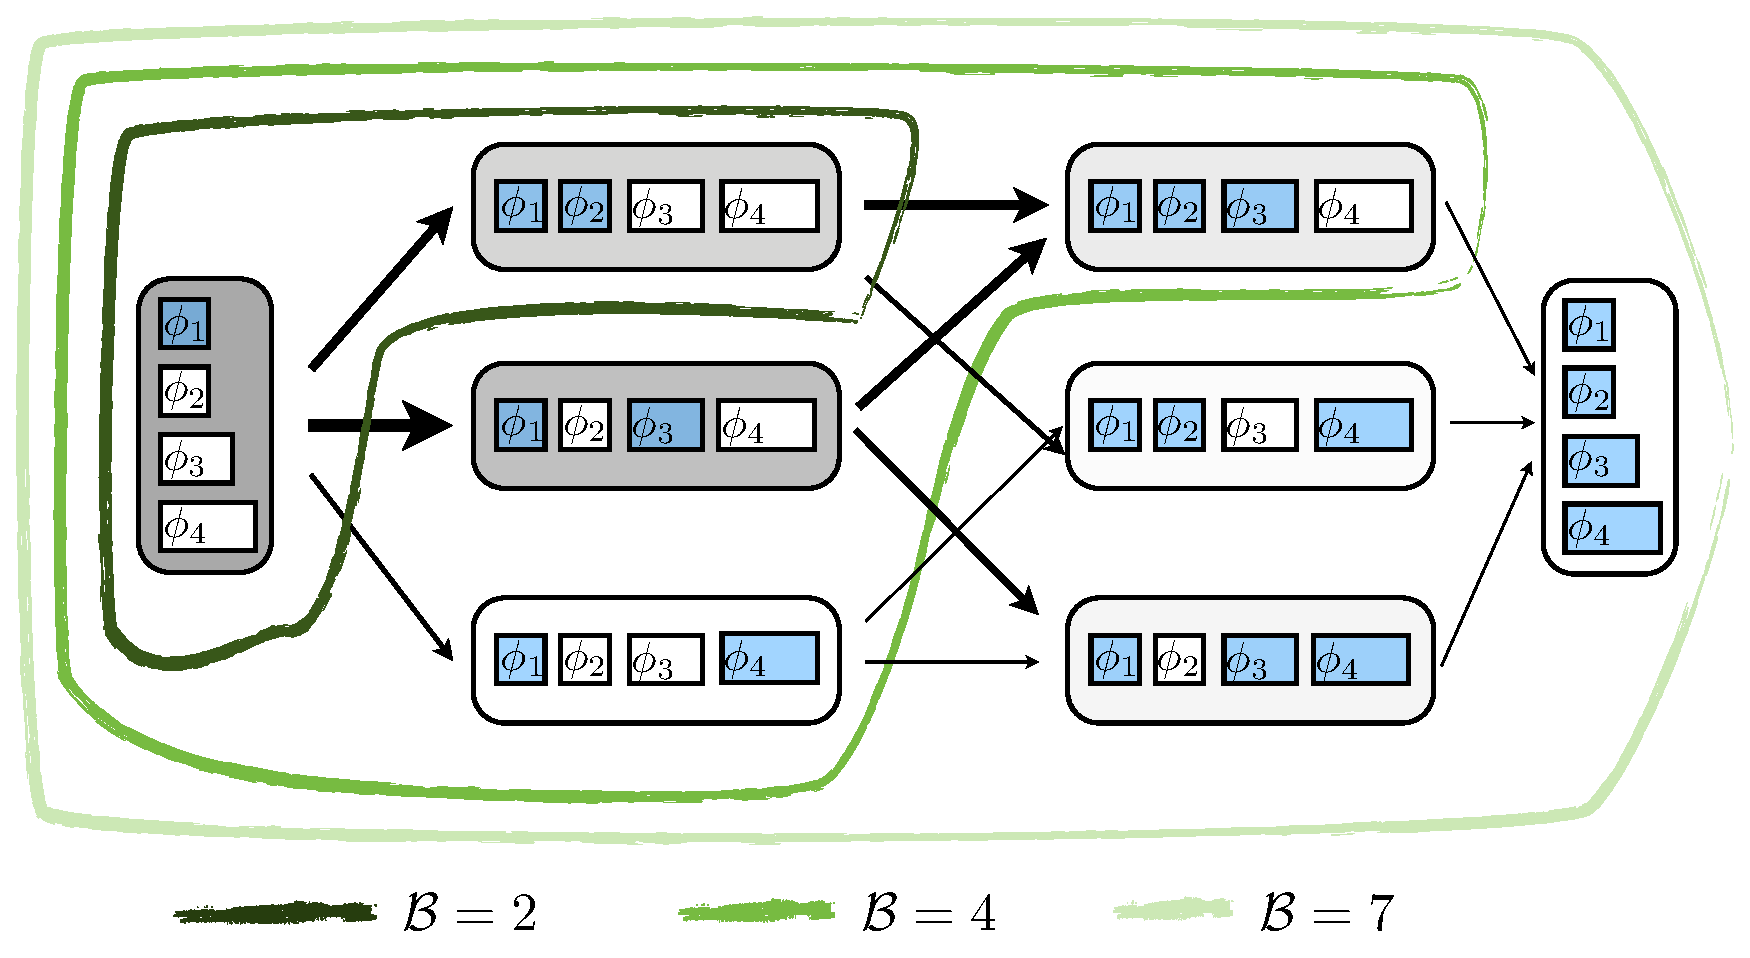
\includegraphics[width=1\linewidth]{../../figures/mdp_masks.pdf}
\caption{
The action space $\mathcal{A}$ of the MDP is the the set of features $\mathcal{H}$, represented by the $\phi$ boxes.
The primary discretization of the state space can be visualized by the possible feature subsets (larger boxes); selected features are colored in the diagram.
The feature selection policy $\pi$ induces a distribution over feature subsets, for a dataset, which is represented by the shading of the larger boxes.
Not all states are reachable for a given budget $\mathcal{B}$.
In the figure, we show three ``budget cuts'' of the state space.
\label{fig:state_space}
}
\end{figure}

\section{Evaluation}
We evaluate the following sequential selection baselines:
\begin{itemize}\addtolength{\itemsep}{-.35\baselineskip}
\item \textbf{Static, greedy}: corresponds to best performance of a policy that does not observe feature values and selects actions greedily ($\gamma=0$).
\item \textbf{Static, non-myopic}: policy that does not observe feature values but uses the MDP machinery with $\gamma=1$ to consider future action rewards.
\item \textbf{Dynamic, greedy}: policy that observed feature values, but selects actions greedily.
% \item \todo{
% \textbf{Active Classification} \parencite{Gao-NIPS-2011}:
% Feature selection is done by greedy selection based on expected information gain divided by cost (so reward is information gain, $\gamma=0$).
% The feature responses are modeled as a mixture of multivariate Gaussians (one mixture element per class label), and inference is instance-specific, akin to locally weighted regression.
% Feature combination is done by the same model: the posteriors are used as the final answers.
% }
% \item
% \todo{\textbf{MD-DAG} \parencite{Benbouzid-ICML-2012}
% Feature selection is done by an MDP policy with three actions: Skip, Evaluate, Quit over a pre-determined sequence of weak learners (unspecified exactly how the sequence is arranged, except ``by quality'').
% }
\end{itemize}
Our method is the \textbf{Dynamic, non-myopic} policy: observed feature values, and full lookahead.

% In addition to the settings above, we evaluate three additional baselines that do not do any selection at all: (a) \textbf{all} features computed; (b) only the \textbf{best} feature (in terms of $\mathcal{G}$) computed; (c) only the \textbf{least costly} feature computed.

In preliminary experiments, Logistic Regression always performed better than the Gaussian Naive Bayes classifier, and so only the former is used in the experiments below.
As described above, we evaluated classification with \textbf{Gaussian} vs. \textbf{Mean} imputation, and with different number of classifiers (1, 3, and 6) clustered by feature subsets.
We found that mean imputation performed better than Gaussian imputation, and although increased number of classifiers sometimes increased performance, it also made our method more prone to overfitting; $K=1$ classifiers worked best on all tasks.
%For reason of space, we report only the best achieved performance in the following evaluation results.

We evaluate two forms of test-time efficient performance measure: the area under the curve and the performance at max budget, although note that all methods are trained only for the former measure.

While the individual implementation details have been largely provided in the preceding text, here we additionally note that some of our policy and classifier implementations use the scikit-learn package \parencite{Pedregosa2011}.

% \subsection{Baselines}
% \paragraph{Active Classification \parencite{Gao-NIPS-2011}}
% Feature selection is done by greedy selection based on expected information gain divided by cost (so reward is information gain, $\gamma=0$).
% The feature responses are modeled as a mixture of multivariate Gaussians (one mixture element per class label), and inference is instance-specific, akin to locally weighted regression.
% Feature combination is done by the same model: the posteriors are used as the final answers.

% \paragraph{Greedy Miser \parencite{Xu-ICML-2012}}
% Feature selection is done by the CART algorithm \parencite{Breiman-1984} with an impurity function that considers feature cost.
% Feature combination is an ensemble of trees.

% \paragraph{MD-DAG \parencite{Benbouzid-2012-ICML}}
% Feature selection is done by an MDP policy with three actions: Skip, Evaluate, Quit over a pre-determined sequence of weak learners (unspecified exactly how the sequence is arranged, except ``by quality'').
% Feature combination is an unweighted sum.

% \paragraph{Timely \parencite{Karayev-NIPS-2012}}
% Feature selection is done by MDP trained using a state feature vector that has the inference output of an MRF combining feature values.
% Feature combination is done by the same MRF.

\begin{figure*}[ht]
\centering
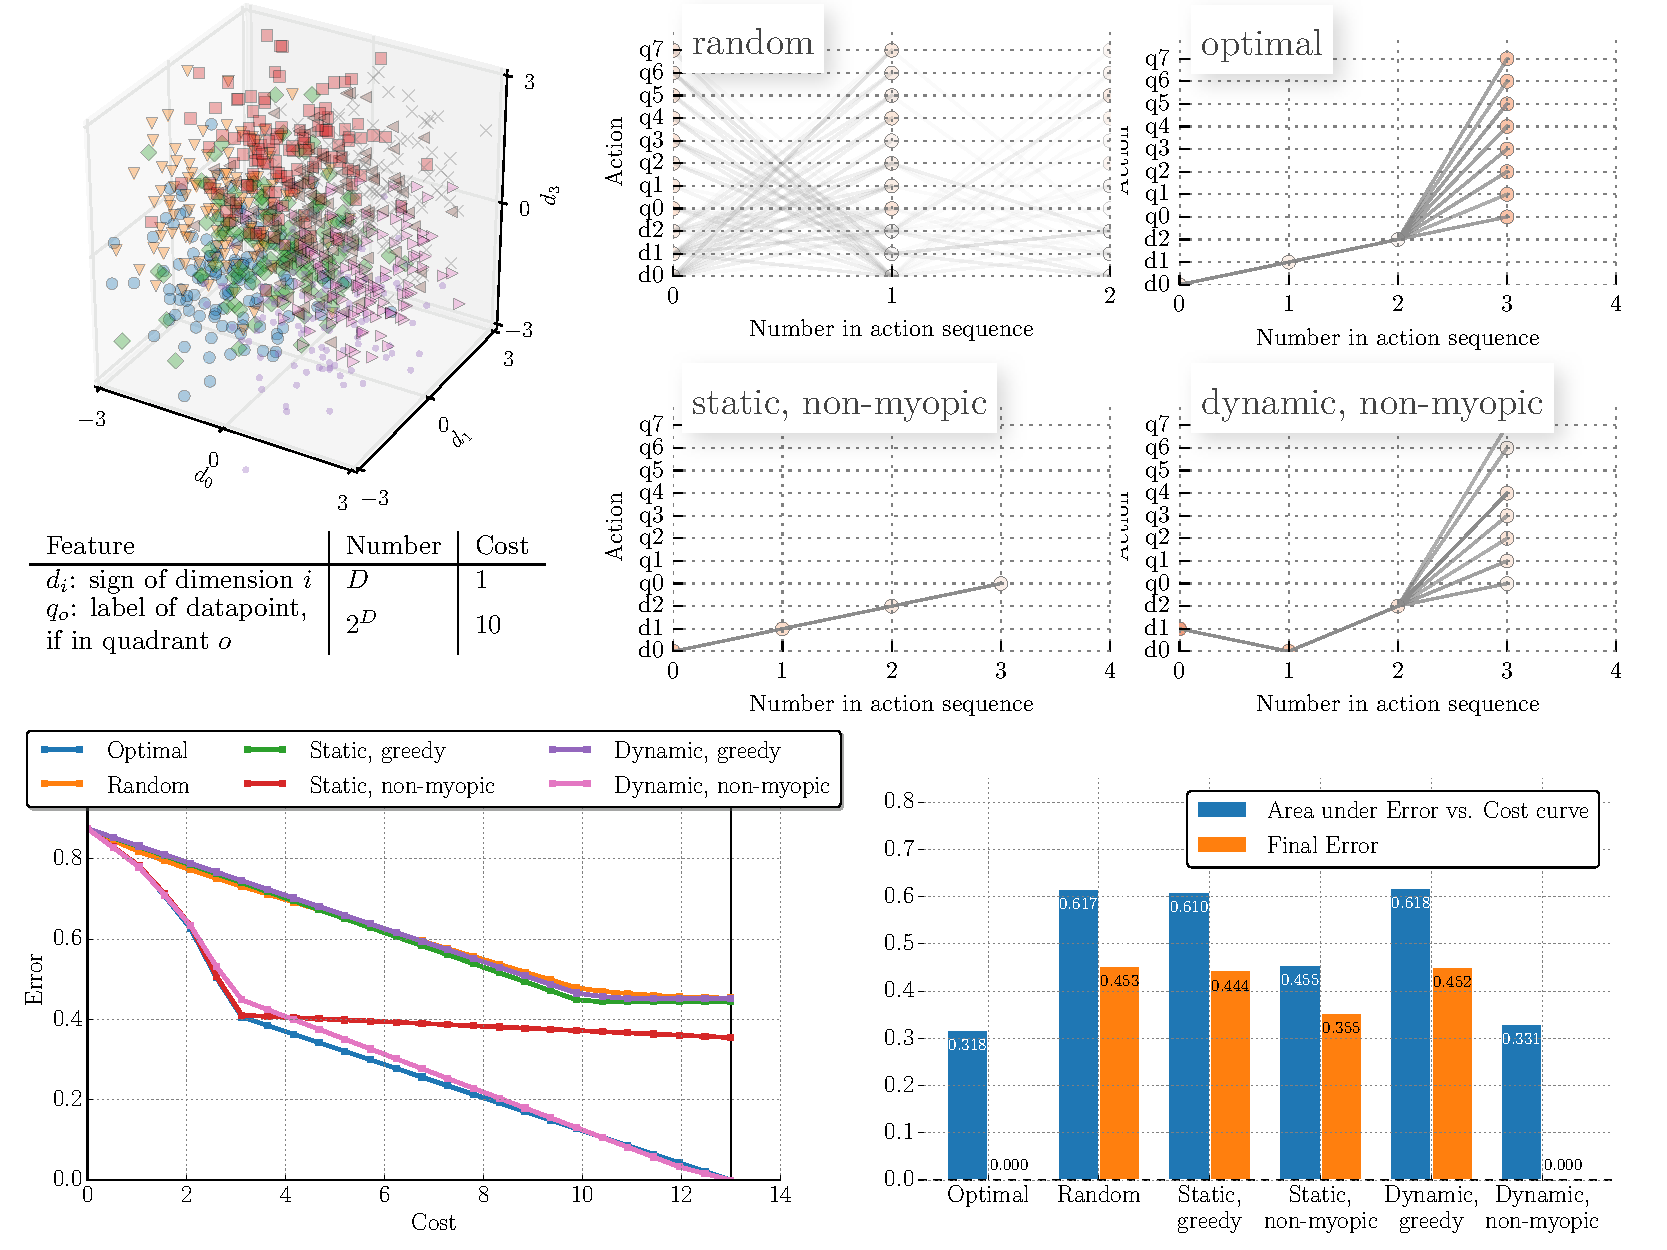
\includegraphics[width=.9\textwidth]{../../figures/synthetic.pdf}
\caption{
Evaluation on the synthetic example (best viewed in color).
The data and the feature costs are shown at top left; the sample feature trajectories of different policies at top right.
(The opacity of the edges corresponds to their prevalence during policy execution; the opacity of the nodes corresponds to the amount of reward obtained in that state.)
Note that the \emph{static, non-myopic} policy correctly learns to select the cheap features first, but is not able to correctly branch, while our \emph{dynamic, non-myopic} approach finds the optimal strategy.
The plots in the bottom half give the error vs. cost numbers.
}

\label{fig:synthetic}
\end{figure*}

\subsection{Synthetic Experiment.}
Following \parencite{Xu-ICML-2013}, we first show that the policy works as advertised in a challenging synthetic example.
In $D$-dimensional space, the data has a label for each of the $2^D$ orthants, and is generated by a unit-variance Gaussian in that orthant (See top left of \autoref{fig:synthetic} for the 3D case).
There are $D$ cheap features that simply return the sign of the data point's coordinate for the corresponding dimension.
For each orthant, there is also an expensive feature that returns the data point's label if the point is located in the corresponding orthant, and random noise otherwise.

The optimal policy on a new data point is to determine its orthant with cheap features, and then take the corresponding expensive action.
Note that both dynamic features and non-myopic learning are crucial to the optimal policy, which is successfully found by our approach.
\autoref{fig:synthetic} shows the results of this optimal policy, a random policy, and of different baselines and our method, trained given the correct minimal budget.

\subsection{Scene recognition.}
The Scene-15 dataset \parencite{Lazebnik-CVPR-2006} contains 4485 images from 15 visual scene classes.
The task is to classify images according to scene.
Following \parencite{Xiao-CVPR-2010}, we extracted 14 different visual features (GIST, HOG, TinyImages, LBP, SIFT, Line Histograms, Self-Similarity, Textons, Color Histograms, and variations).
The features vary in cost from 0.3 seconds to 8 seconds, and in single-feature accuracy from 0.32 (TinyImages) to .82 (HOG).
Separate multi-class linear SVMs were trained on each feature channel, using a random 100 positive example images per class for training.
We used the \texttt{liblinear} implementation, and K-fold cross-validated the penalty parameter $C$.
The trained SVMs were evaluated on the images not used for training, resulting in a dataset of 2238 vectors of 210 confidence values: 15 classes for each of the 14 feature channels.
This dataset was split 60-40 into training and test sets for our experiments.

\hyperref[fig:scenes]{Figure~\ref*{fig:scenes}} shows the results, including learned policy trajectories.
For all evaluated budgets, our \emph{dynamic, non-myopic} method outperforms all others on the area under the error vs. cost curve metric.
Our results on this dataset match the reported results of Active Classification \parencite{Gao-NIPS-2011} (Figure 2) and Greedy Miser \parencite{Xu-ICML-2012} (Figure 3), although both methods use an additional powerful feature channel (ObjectBank)\footnote{Detailed results for this and other experiments are on the project page (see front page for the \href{http://sergeykarayev.com/recognition-on-a-budget/}{link}).}.


\subsection{ImageNet and maximizing specificity.}
The full ImageNet dataset has over 10K categories and over a million images \parencite{Deng-ECCV-2010}.
The classes are organized in a hierarchical structure, which can be exploited for novel recognition tasks.
We evaluate on a 65-class subset introduced in ``Hedging Your Bets'' \parencite{Deng-CVPR-2012}.
In this evaluation, we consider the situation where the initial feature computation has already happened, and the task is to find a path through existing one-vs-all classifiers: features correspond to Platt-scaled SVM confidences of leaf-node classifiers (trained on SIFT-LLC features), and each has cost 1 \parencite{Deng-ECCV-2010}.
Following \parencite{Deng-CVPR-2012}, accuracy is defined on all nodes, and inner node confidences are obtained by summing the probabilities of the descendant nodes.

We combine our sequential feature selection with the ``Hedging Your Bets'' method for backing off prediction nodes using the ImageNet hierarchy to maintain guaranteed accuracy while giving maximally specific answers, given a cost budget.
The results are given in \hyperref[fig:imagenet]{Figure~\ref*{fig:imagenet}}.
As the available budget increases, the \emph{specificity} (defined by normalized information gain in the hierarchy) of our predictions also increases, while accuracy remains constant.
Visualizing this on the ILSVRC-65 hierarchy, we see that the fraction of predictions at the leaf nodes grows with available computation time.
This formulation presents a novel angle on modeling the time course of human visual perception.

\begin{figure*}[ht]
\centering
    \centering
    \begin{subfigure}[b]{0.39\textwidth}
            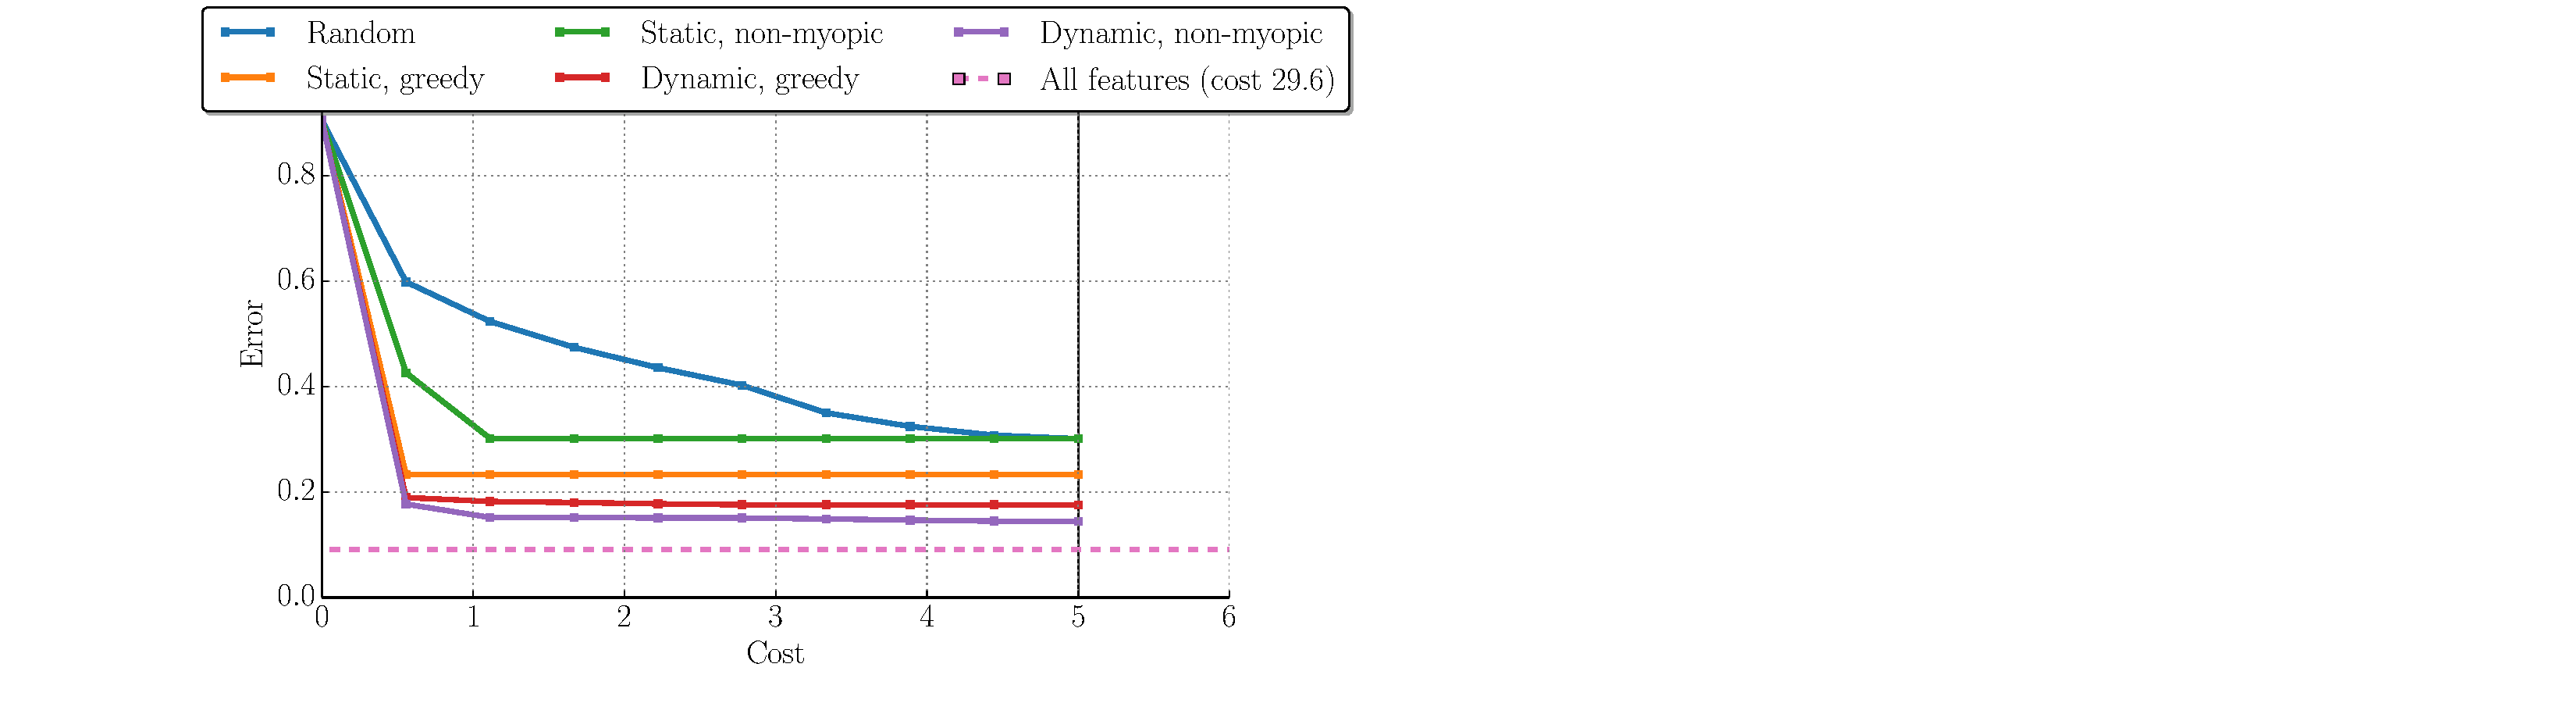
\includegraphics[width=\textwidth]{../../figures/apr11_assembly/scene_15_5_crop.pdf}
            \caption{Error given by policies learned for a budget = 5.}
    \end{subfigure}%
    \begin{subfigure}[b]{0.36\textwidth}
            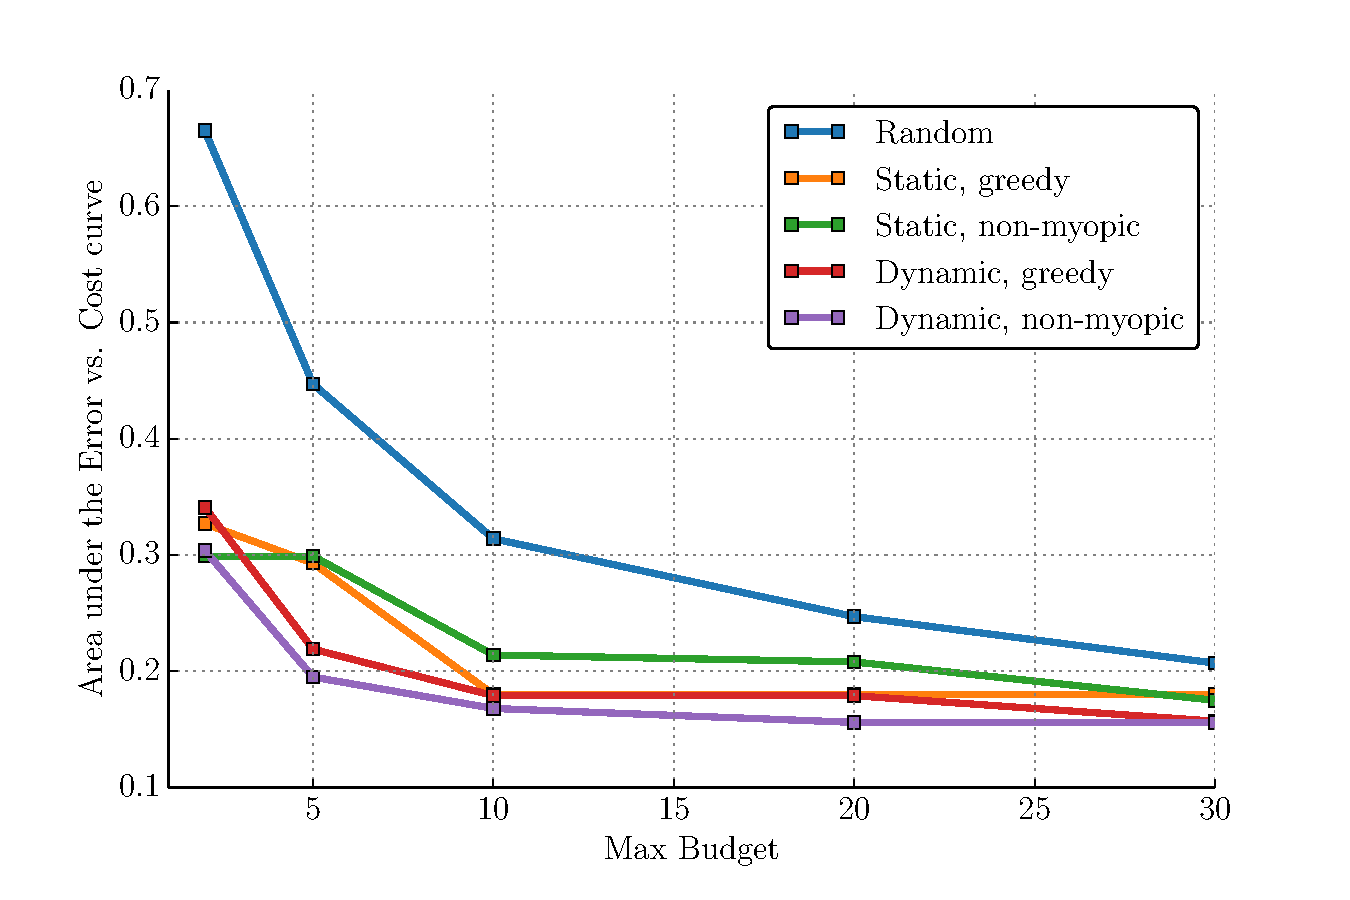
\includegraphics[width=\textwidth]{../../figures/apr11_assembly/_scenes15_auc.pdf}
            \caption{Areas under error vs. cost curves of policies learned at different budgets.}
    \end{subfigure}%
    \begin{subfigure}[b]{0.25\textwidth}
            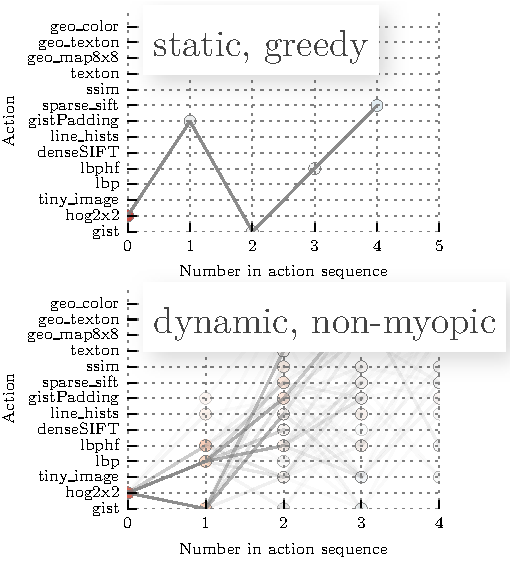
\includegraphics[width=\textwidth]{../../figures/apr11_assembly/scenes_result.pdf}
            \caption{Policy trajectories.}
    \end{subfigure}

    \caption{
Results on Scenes-15 dataset (best viewed in color).
Figure (a) shows the error vs. cost plot for policies learned given a budget of 5 seconds.
Figure (b) aggregates the area under the error vs. cost plot metrics for different policies and budgets, showeing that our approach outperforms baselines no matter what budget it's trained for.
Figure (c) shows the branching behavior of our dynamic policy.
\label{fig:scenes}
    }
\end{figure*}
\begin{figure*}[ht]
\centering
    \begin{subfigure}[b]{0.52\textwidth}
            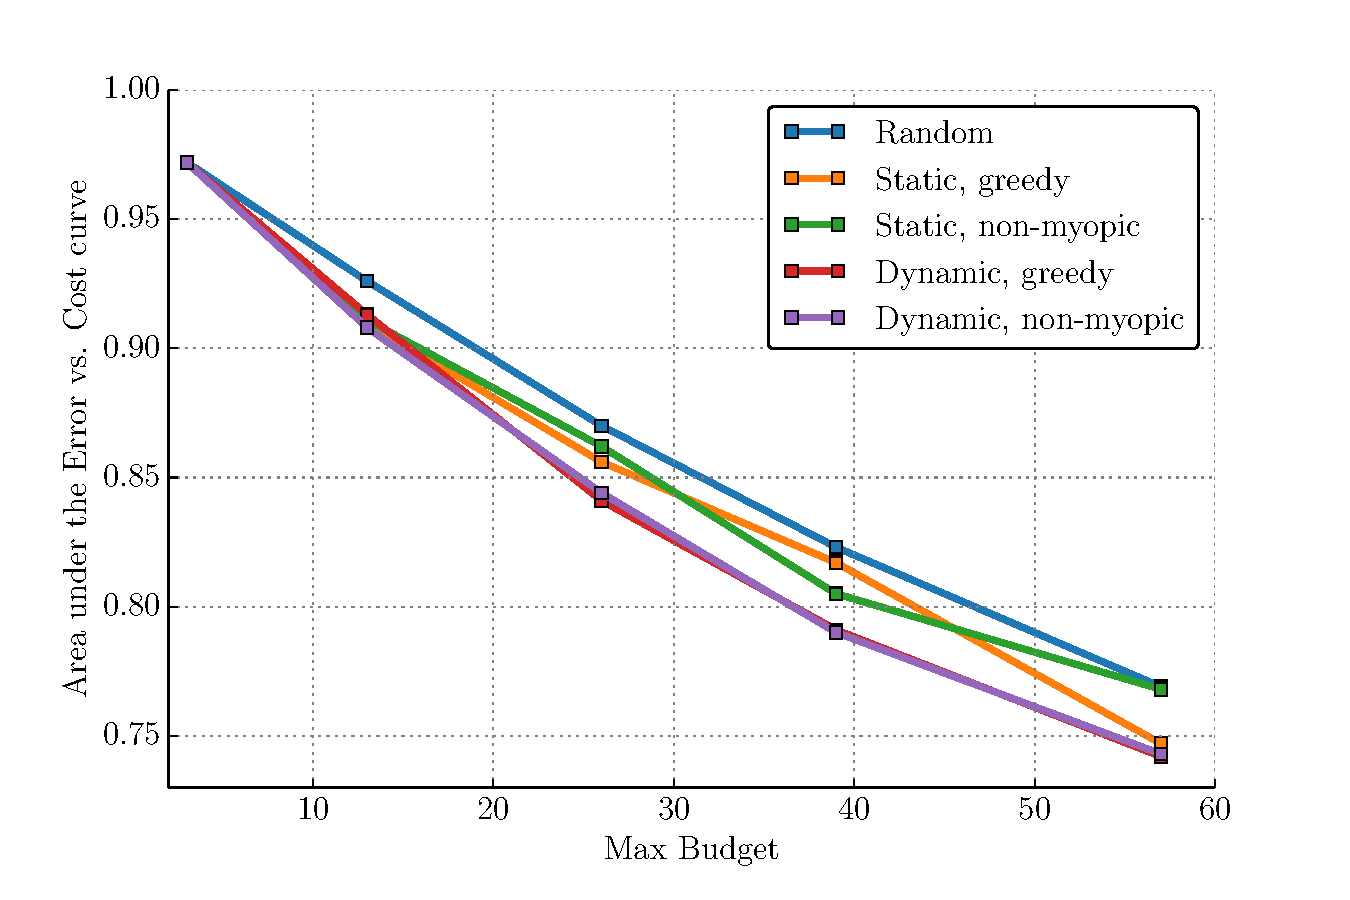
\includegraphics[width=\textwidth]{../../figures/apr11_assembly/_ilsvrc65_auc.pdf}
            \caption{
            Areas under error vs. cost curves for policies learned at different budgets.
            (No specificity back-off is performed here).
            \label{fig:imagenet-a}
            }
    \end{subfigure}\hfill%
    \begin{subfigure}[b]{0.43\textwidth}
            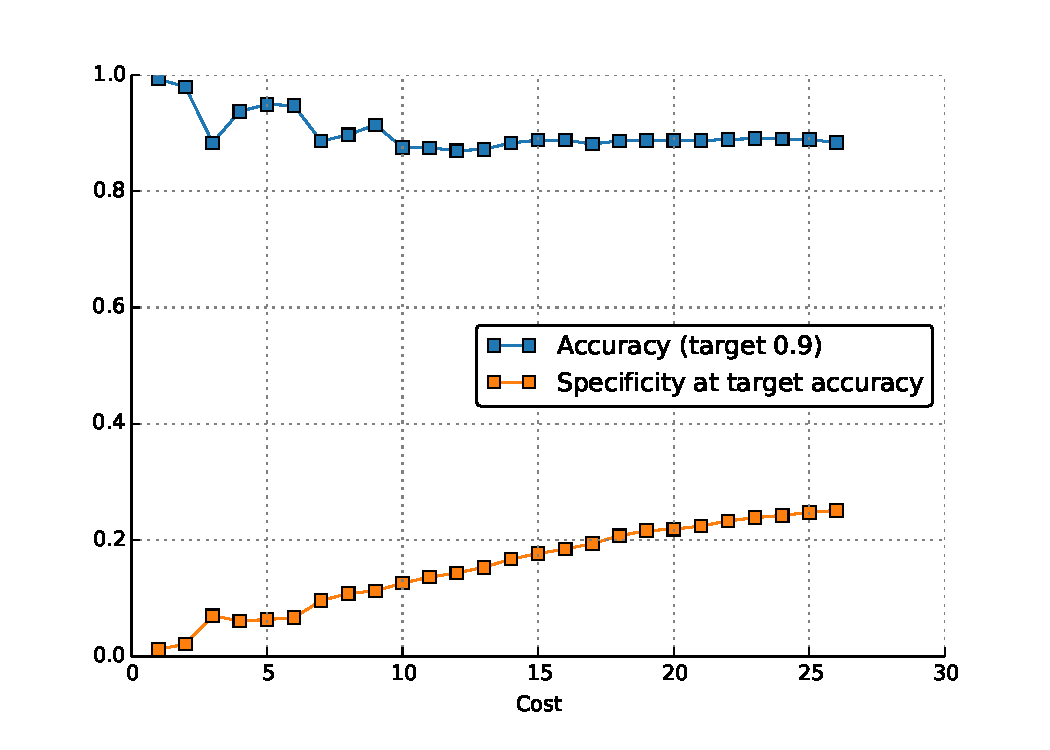
\includegraphics[width=\textwidth]{../../figures/apr11_assembly/ilsvrc65_acc.pdf}
            \caption{
            Holding prediction accuracy constant, we achieve increased specificity with increased cost (on \emph{Dynamic, non-myopic} policy, budget = 36).
            \label{fig:imagenet-b}
            }
    \end{subfigure}\\\vspace{1em}
    \begin{subfigure}[b]{.97\textwidth}
            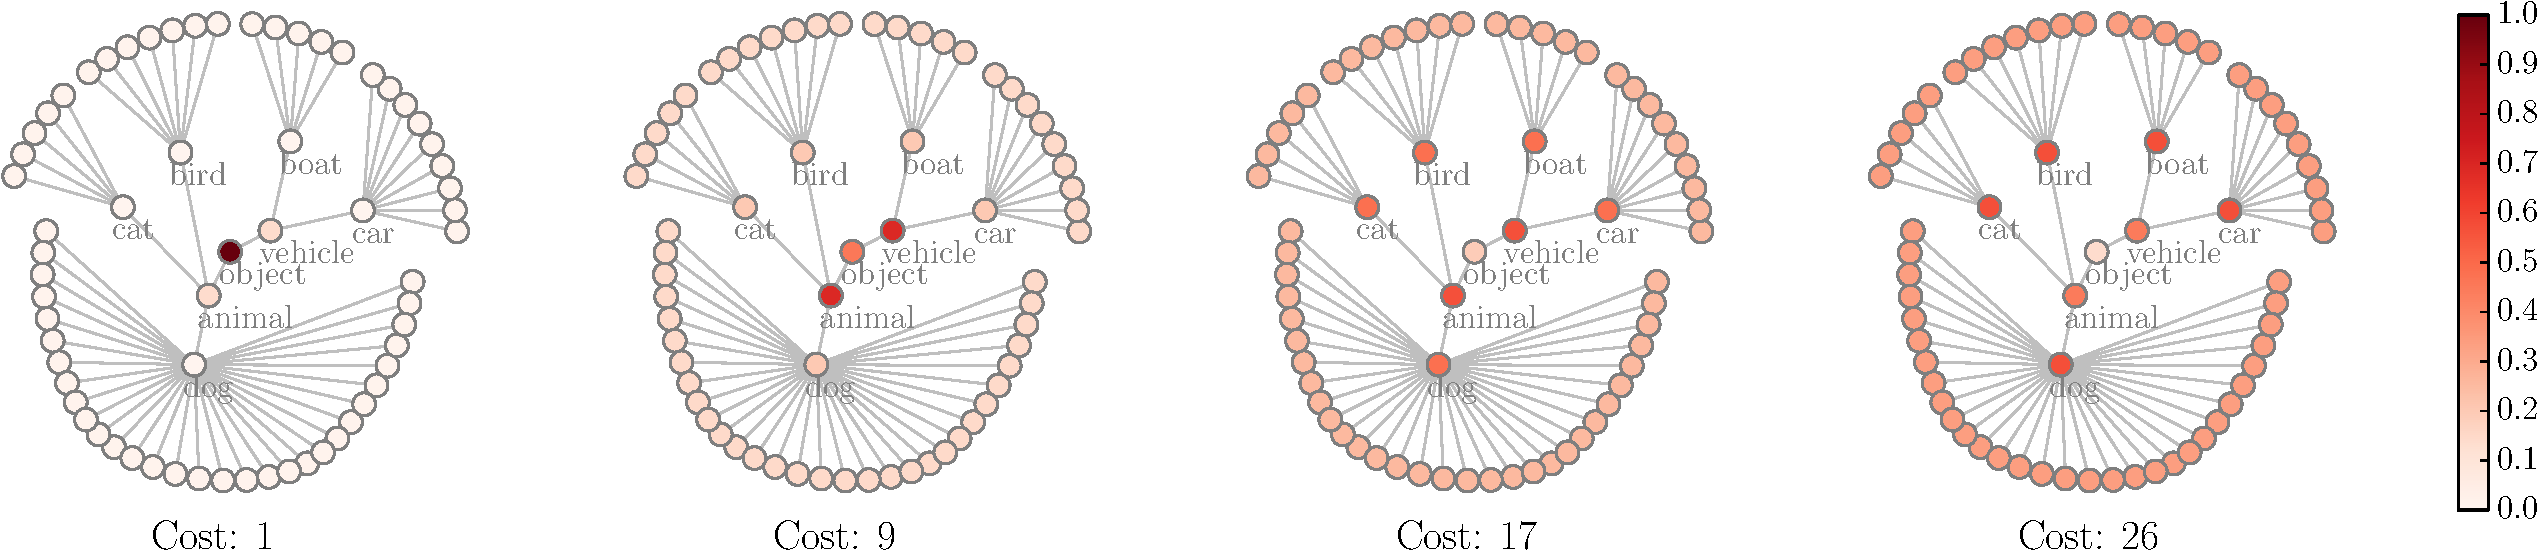
\includegraphics[width=\textwidth]{../../figures/apr11_assembly/ilsvrc65_network-crop.pdf}
            \caption{
            We visualize the fraction of predictions made at inner vs. leaf nodes of ILSVRC-65 at different cost points of an Anytime policy: with more computation, accurate predictions are increasingly made at the leaf nodes.
            \label{fig:imagenet-c}
            }
    \end{subfigure}

\caption{
Results on the ILSVRC-65 dataset (best viewed in color).
Figure (a) shows our dynamic approaches outperforming static baselines for all practical cost budgets.
When our method is combined with Hedging Your Bets \parencite{Deng-CVPR-2012}, a constant prediction accuracy can be achieved at all points in the Anytime policy, with \emph{specificity} of predictions increasing with the cost of predictions.
Figures (b) and (c) show this for the \emph{dynamic, non-myopic} policy learned for budget = 26.
This is analogous to human visual performance, which shows increased specificity at longer stimulus times.
\label{fig:imagenet}}
\end{figure*}

%!TEX root=paper/paper.tex
\chapter{Prediction with Features Missing at Test Time}

\section{Abstract}
We look at prediction with all features available at training time, but only a subset observed at test time.
Such situations may arise due to sensor loss, or when using test-time instance-specific feature selection.
We examine three areas of modeling choices:

\begin{enumerate}
\item For imputation, we look at mean, SVD, joint Gaussian conditioning, and nearest neighbor methods.

\item For classification, we evaluate augmenting the training data with imputed values, modifying the loss function to consider the expected feature ``corruption'', and using non-linear classifiers.

\item We additionally evaluate training different classifiers for different subsets of observed features.
\end{enumerate}

We evaluate reconstruction and classification error on two datasets: Digits and Scenes-15.
Two feature selection policies are considered: Random and Clustered.
For each policy, we consider Independent and Block-wise selection patterns.

We find that mean imputation with classifier retraining is a reasonably well-performing approach.
Nearest Neighbor methods perform best but are the most expensive.
Gaussian imputation method performs very well, but is also expensive.

Training classifiers with a loss function modified to expect a certain level of feature corruption did not improve performance.
Training additional classifiers for clusters of observed feature subsets did not improve performance.

\section{Introduction}
In supervised prediction problems, \emph{features} extracted from inputs are combined to output a real value (regression) or a label (classification).
The goal of training is to minimize the \emph{loss} of the predictions with the true values or labels---for example, the accuracy of classification.

We look at a complication of this problem.
While all features are available at training time, only a subset of features of each instance is observed at test time.
Such situations can arise in real world deployments of predictive systems due to sensor failure.
Another motivation for the problem comes from work on dynamic feature selection: to predict with minimum loss on a fixed time budget, different subsets of features are extracted for different instances \parencite{Karayev-NIPS-2012, Xu-ICML-2013}.

Since the training set is fully observed, we can train a classifier with all features.
At test time, we could attempt to impute the unobserved feature values given the observed ones, and use the classifier trained on the fully observed training set.
There are many methods of imputing missing values, differing in their power and cost.
We consider: simple mean imputation; singular value decomposition-based imputation; multivariate Gaussian conditioning; and nearest neighbor imputation with two similarity measures.

In addition to imputing at test time, we can apply the test-time observation process to the training data, impute values, and re-train the classifier.
This amounts to a regularization that prevents the classifier from relying on any single feature, as it may not be in the observed subset.
Taking this idea further, we could work the expected feature ``corruption'' into the loss function of the linear classifier, which is equivalent to augmenting the training set with an infinite amount of corrupted data.

The feature selection process may not select features independently.
It could select features by block instead of one by one, and it could have a bound on the total number of unique subsets that are selected.
We evaluate in these conditions, and notice that if there is a small bound on the number of subsets, then we can learn a separate classifier for each subset of observed features.
Even if the bound is not small, we may still derive benefit from training more than one classifier, and at test time using the classifier trained on the closest subset of features to the observed instance.

\section{Problem Formulation}

\begin{mydef} \label{def:problem}
\textbf{The prediction problem} consists of
\begin{itemize}
\item Set $\mathcal{D}$ of $N$ instances of $K$ possible labels: $\mathcal{D} = \{x_n \in \mathcal{X}, y_n \in \{1, \dots, K\}\}_{n=1}^N$.

\item Set $\mathcal{H}$ of $F$ features $\mathcal{H} = \{h_f : \mathcal{X} \mapsto \mathbb{R} \}_{f=1}^F$.\\
To represent featurized instance, we write $\mathbf{x} = [h_0(x), h_1(x), \dots, h_f(x)]$.

\item Test-time feature selection function $o(x, b): \mathcal{X} \times \mathbb{R} \mapsto \mathbb{B}^F$, where $\mathbb{B} \in \{0, 1\}$, and $b \in [0, 1]$ is given and specifies the fractional selection \emph{budget}.

\item Loss function $\ell(g(x), y): \mathbb{R}^K \times \{1, \dots, K\} \mapsto \mathbb{R}$.
\end{itemize}

Given $b$, we seek a procedure $g(x)$ that minimizes total loss $\sum \ell(g(x_n), y_n)$ under the condition that $o(x, b)$ is applied to each $x$.
\end{mydef}

Applied to $x$, $o(x, b)$ gives the binary selection vector $\mathbf{o}$ which splits $\mathbf{x}$ it into observed and unobserved parts such that $\mathbf{x}^m = [\mathbf{x}^\text{o}, \mathbf{x}^\text{u}]$.

$X^c$ denotes the fully observed $N \times F$ training set.
We assume that we have only sequential access to the missing-feature test instances $\mathbf{x}^m$.

We see three experimental conditions: (1) how to fill in missing values; (2) which loss function to use in learning the classifier and whether to augment the training data; (3) how many classifiers to learn.


\section{Classifiers}

In addition to the $k$-NN classifier described above, we consider three linear classifiers, obtained by minimizing:
\begin{enumerate}
  \item Logistic loss on fully observed data: simply using $X^c$.
  \item Logistic loss on synthetically re-imputed version of the data: we obtain $X^m$ through applying $o(x, b)$ on each $x^c$, and then imputing the missing values with the methods described.
  \item Logistic and quadratic loss derived with Marginalized Corrupted Features (MCF) \parencite{Maaten-ICML-2013}.
\end{enumerate}

The idea of (3) is to move the expectation of feature corruption into the loss function, which is equivalent to adding an infinite amount of corrupted data to the training set.
Remarkably, this is not any more computationally complex than the standard loss (although minimization does take longer, empirically).

For example, for blankout noise and logistic loss, we can derive the surrogate loss
\begin{equation}
\mathcal{L}(D; \mathbf{\theta}) \leq \sum_{n=1}^N \log \left( 1 + \prod_{f=1}^F \left[ q_f + (1 - q_f) e^{-y_n \theta_f \frac{1}{1 - q_d} x_{nf}} \right] \right)
\end{equation}

For additional loss functions, see \parencite{Maaten-ICML-2013}.

\subsection{Clustering classifiers}

\section{Evaluation}





% %!TEX root=paper/thesis.tex
\chapter{Cascaded CNN recognition}

\gray{Lorem ipsum Labore aute minim sed pariatur amet sunt id proident tempor culpa incididunt ut Ut Duis fugiat tempor cupidatat aliqua sint reprehenderit amet in fugiat irure dolor laborum commodo est cupidatat ullamco ut qui dolor dolor est adipisicing culpa eiusmod et commodo culpa in eu irure magna in irure aliquip sint cupidatat sint deserunt laborum sint ad quis sed sunt ut deserunt pariatur sed mollit officia dolore Excepteur aute culpa pariatur aute proident magna incididunt reprehenderit cillum ea Excepteur in ad tempor amet ea elit in est ad quis tempor aliquip deserunt consectetur dolor dolore aute culpa sed magna ullamco ut pariatur ea et occaecat commodo ullamco sed sit eu Duis mollit dolore officia est officia in occaecat consequat dolor sunt proident eu in in ea velit qui quis nulla ad eiusmod sed in qui ex ex in tempor exercitation elit do tempor aliquip elit officia aute incididunt Excepteur fugiat cupidatat ad commodo consequat et commodo adipisicing proident est sit elit adipisicing amet dolore do eu adipisicing ullamco et ea ex irure reprehenderit magna velit aute sed laborum Ut do aute adipisicing quis dolore eiusmod sed elit ad commodo adipisicing reprehenderit eiusmod nulla mollit sint minim adipisicing ullamco adipisicing anim sit aute veniam esse nisi aute deserunt culpa Ut reprehenderit in sed occaecat reprehenderit cillum do cupidatat veniam est dolore aliquip.}

% %!TEX root=paper/paper.tex
\chapter{Conclusion}\label{sec:conclusion}

\PM{Contribution}
We note a significant problem that has received little research attention: Anytime visual recognition.
The problem is motivated by the properties of human visual perception and by the need to effectively schedule computationally expensive state-of-the-art computer vision methods for different computational budgets.
We approach the problem from the perspective of reinforcement learning, and successfully learn fully general policies for selecting detector and classifier actions.
To evaluate our approaches, we introduce a new metric of Anytime performance, based on the area of performance vs. cost curve.
In all experiments, we show that having a dynamic state (allowing closed-loop policies) and planning ahead increases performance.

\PM{Detection}
We present a method for learning ``closed-loop'' policies for multi-class object detection, given existing object detectors and classifiers and a metric to optimize.
The method learns the optimal policy using reinforcement learning, by observing execution traces in training.
As always with reinforcement learning problems, defining the reward function requires some manual work.
Here, we derive it for the novel detection AP vs. Time evaluation that we suggest is useful for evaluating efficiency in recognition.
If detection on an image is cut off after only half the detectors have been run, our method does $66\%$ better than a random ordering, and $14\%$ better than an intelligent baseline.
In particular, our method learns to take action with no intermediate reward in order to improve the overall performance of the system.

\PM{Classification}
For the classification task, we additionally need to train classifiers for partially-observed sets of features.
We investigate methods such as different forms of imputation and classifier clustering for this task, and adjust the reward function and the featurization of the state.
We show improved Anytime performance on one synthetic classification task and two real visual recognition tasks using our method.
On a hierarchically-structured dataset, we additionally show that accuracy of predictions can be held constant for all budgets, while the specificty of predictions increases.

\PM{C-CNN}
We first consider approaches which can effectively reorder the sequence of regions to maximize the chance that correct detections will be found early, based on inference from relatively lightweight features.
We show that basic strategies, such as simply randomly reordering the boxes such that they do not have a degenerate spatial layout, provides a surprising boost, and that very simple features such as region and gradient statistics can effectively prioritize regions.
The main contribution, however, is the Cascaded CNN model, which adds a novel Reject layer to the AlexNet architecture and obtains an almost 10x speedup of the R-CNN detection method with only a 10\% degradation of state-of-the-art performance on PASCAL VOC detection.

\section{Future work}

\PM{Decisions}
Although computation devoted to scheduling actions is less significant than the computation due to running the actions in all of our work, our framework does not explicitly consider this decision-making cost.
A welcome extension would explicitly model this, perhaps drawing on eixsting theoretical work on meta-reasoning \parencite{Hay2012}.
This principle can also be applied to neural networks; we currently learn rejection thresholds in a process separate from the CNN training.
Future work should learn these thresholds jointly with the convolutional filters and the rest of the network layers.

\PM{Classification}
Nearest-neighbor method work really well for settings with partially observed sets of features, but were too slow in our evaluation.
Locality-sensitive hashign methods may provide an effective solution.
In particular, the method of \cite{Gao-NIPS-2011} could be valuably extended with hashing to maintain its model-free advantages at an acceptable speed.

\PM{Perception}
Beyond the aspects of practical deployment of vision systems that our work is motivated by, we are curious to further investigate our model as a tool to study human cognition and the time course of visual perception.
Only a few attempts have been made to explain this: for example, via sequential decision processes in \textcite{Hegde-Neuro-2008}.
While we have not made any claims about the biological mechanism of perception, our work in reinforcement learning-based feature selection as well as convolutional neural networks has explanatory potential if more tightly integrated in future work.


% \appendix
% \chapter{../definitions}

\printbibliography
\end{document}
